%% Results and discussion
%%=========================================

\chapter{Results and Discussion}
\label{ch:results}
This chapter presents the results of the experiments we conducted. Section \ref{sec:accuracy_on_datasets_results} presents the results of the experiment with three datasets of various sizes. The results of the experiment with two fonts are presented in Section \ref{sec:handling_of_two_fonts}. In Section \ref{sec:noise_handling} we present the results of the {\tt EncDecAtt} model's robustness to noise. The final ``stress test'' results are presented in Section \ref{sec:stress_test}, and all the results are discussed in Section \ref{sec:result_discussion}. Finally, in Section \ref{sec:reasoning} we analyze the models in the context of our results.

%%=========================================

\section{Accuracy on Datasets}
\label{sec:accuracy_on_datasets_results}
Table \ref{table:accuracy_model_data_sets} contains the accuracy for each model on each of the three datasets of various sizes. The accuracy and loss plots for each test are presented next, showing the progression over the epochs.

\begin{table}[h]
    \centering
    \begin{tabular}{|l|l|l|l|}
        \hline 
                                        & \textbf{Small dataset}          & \textbf{Medium dataset}         & \textbf{Big dataset}            \\ \hline
        {\tt VecRep }                   & 16.80\%                         & 25.14\%                         & 55.01\%                         \\ \hline
        {\tt EncDecReg}                 & 41.20\%                         & 55.52\%                         & 95.49\%                         \\ \hline
        {\tt EncDecAtt}                 & \textbf{92.00\%}                & \textbf{97.16\%}                & \textbf{98.75\%}                \\ \hline
    \end{tabular}
    \captionsetup{justification=centering}
    \caption{Test accuracy for each model on each test set, with the best results for each test set in bold}
    \label{table:accuracy_model_data_sets}
\end{table}

The {\tt EncDecAtt} model had the best results on all three datasets. The lowest accuracy this model had was 92\% on the smallest dataset. Across all three datasets, the difference between the best and worst results for the {\tt EncDecAtt} model was less than 7\%. These results are in contrast to the {\tt EncDecReg} model, which had low accuracy results for both the small and medium datasets, but high accuracy on the big dataset. The {\tt EncDecReg} model had an accuracy of almost 95.5\% on the big dataset, which is less than 4\% worse than the results for the {\tt EncDecAtt} model. The difference in the accuracy between the {\tt EncDecReg} and {\tt EncDecAtt} model on the medium dataset was more than 40\% and almost 50\% on the smallest dataset. The {\tt VecRep} model had consistently lower accuracy than the two other but almost doubled its accuracy from the medium to the big dataset.

\subsection{VecRep}
\subsubsection{Accuracy and Loss}
\resultplots{fig/results/experiment1/small/vecrep/}{plot_accuracy.png}{plot_loss.png}{result1_small_vecrep}{Accuracy and loss for {\tt VecRep} on small dataset}{ht}
\resultplots{fig/results/experiment1/medium/vecrep/}{plot_accuracy.png}{plot_loss.png}{result1_medium_vecrep}{Accuracy and loss for {\tt VecRep} on medium dataset}{hp}
\newpage
\resultplots{fig/results/experiment1/big/vecrep/}{plot_accuracy.png}{plot_loss.png}{result1_big_vecrep}{Accuracy and loss for {\tt VecRep} on big dataset}{ht}

The minimal increase in accuracy for all three {\tt VecRep} models across the epochs indicates that the model was unable to learn. The loss values for the tests on the small and medium datasets seem to decrease during the first couple of epochs, while the loss value for the test on the big dataset appears highly erratic.

\newpage
\subsubsection{Confusion Matrix}
\begin{figure}[h]
    \centering
    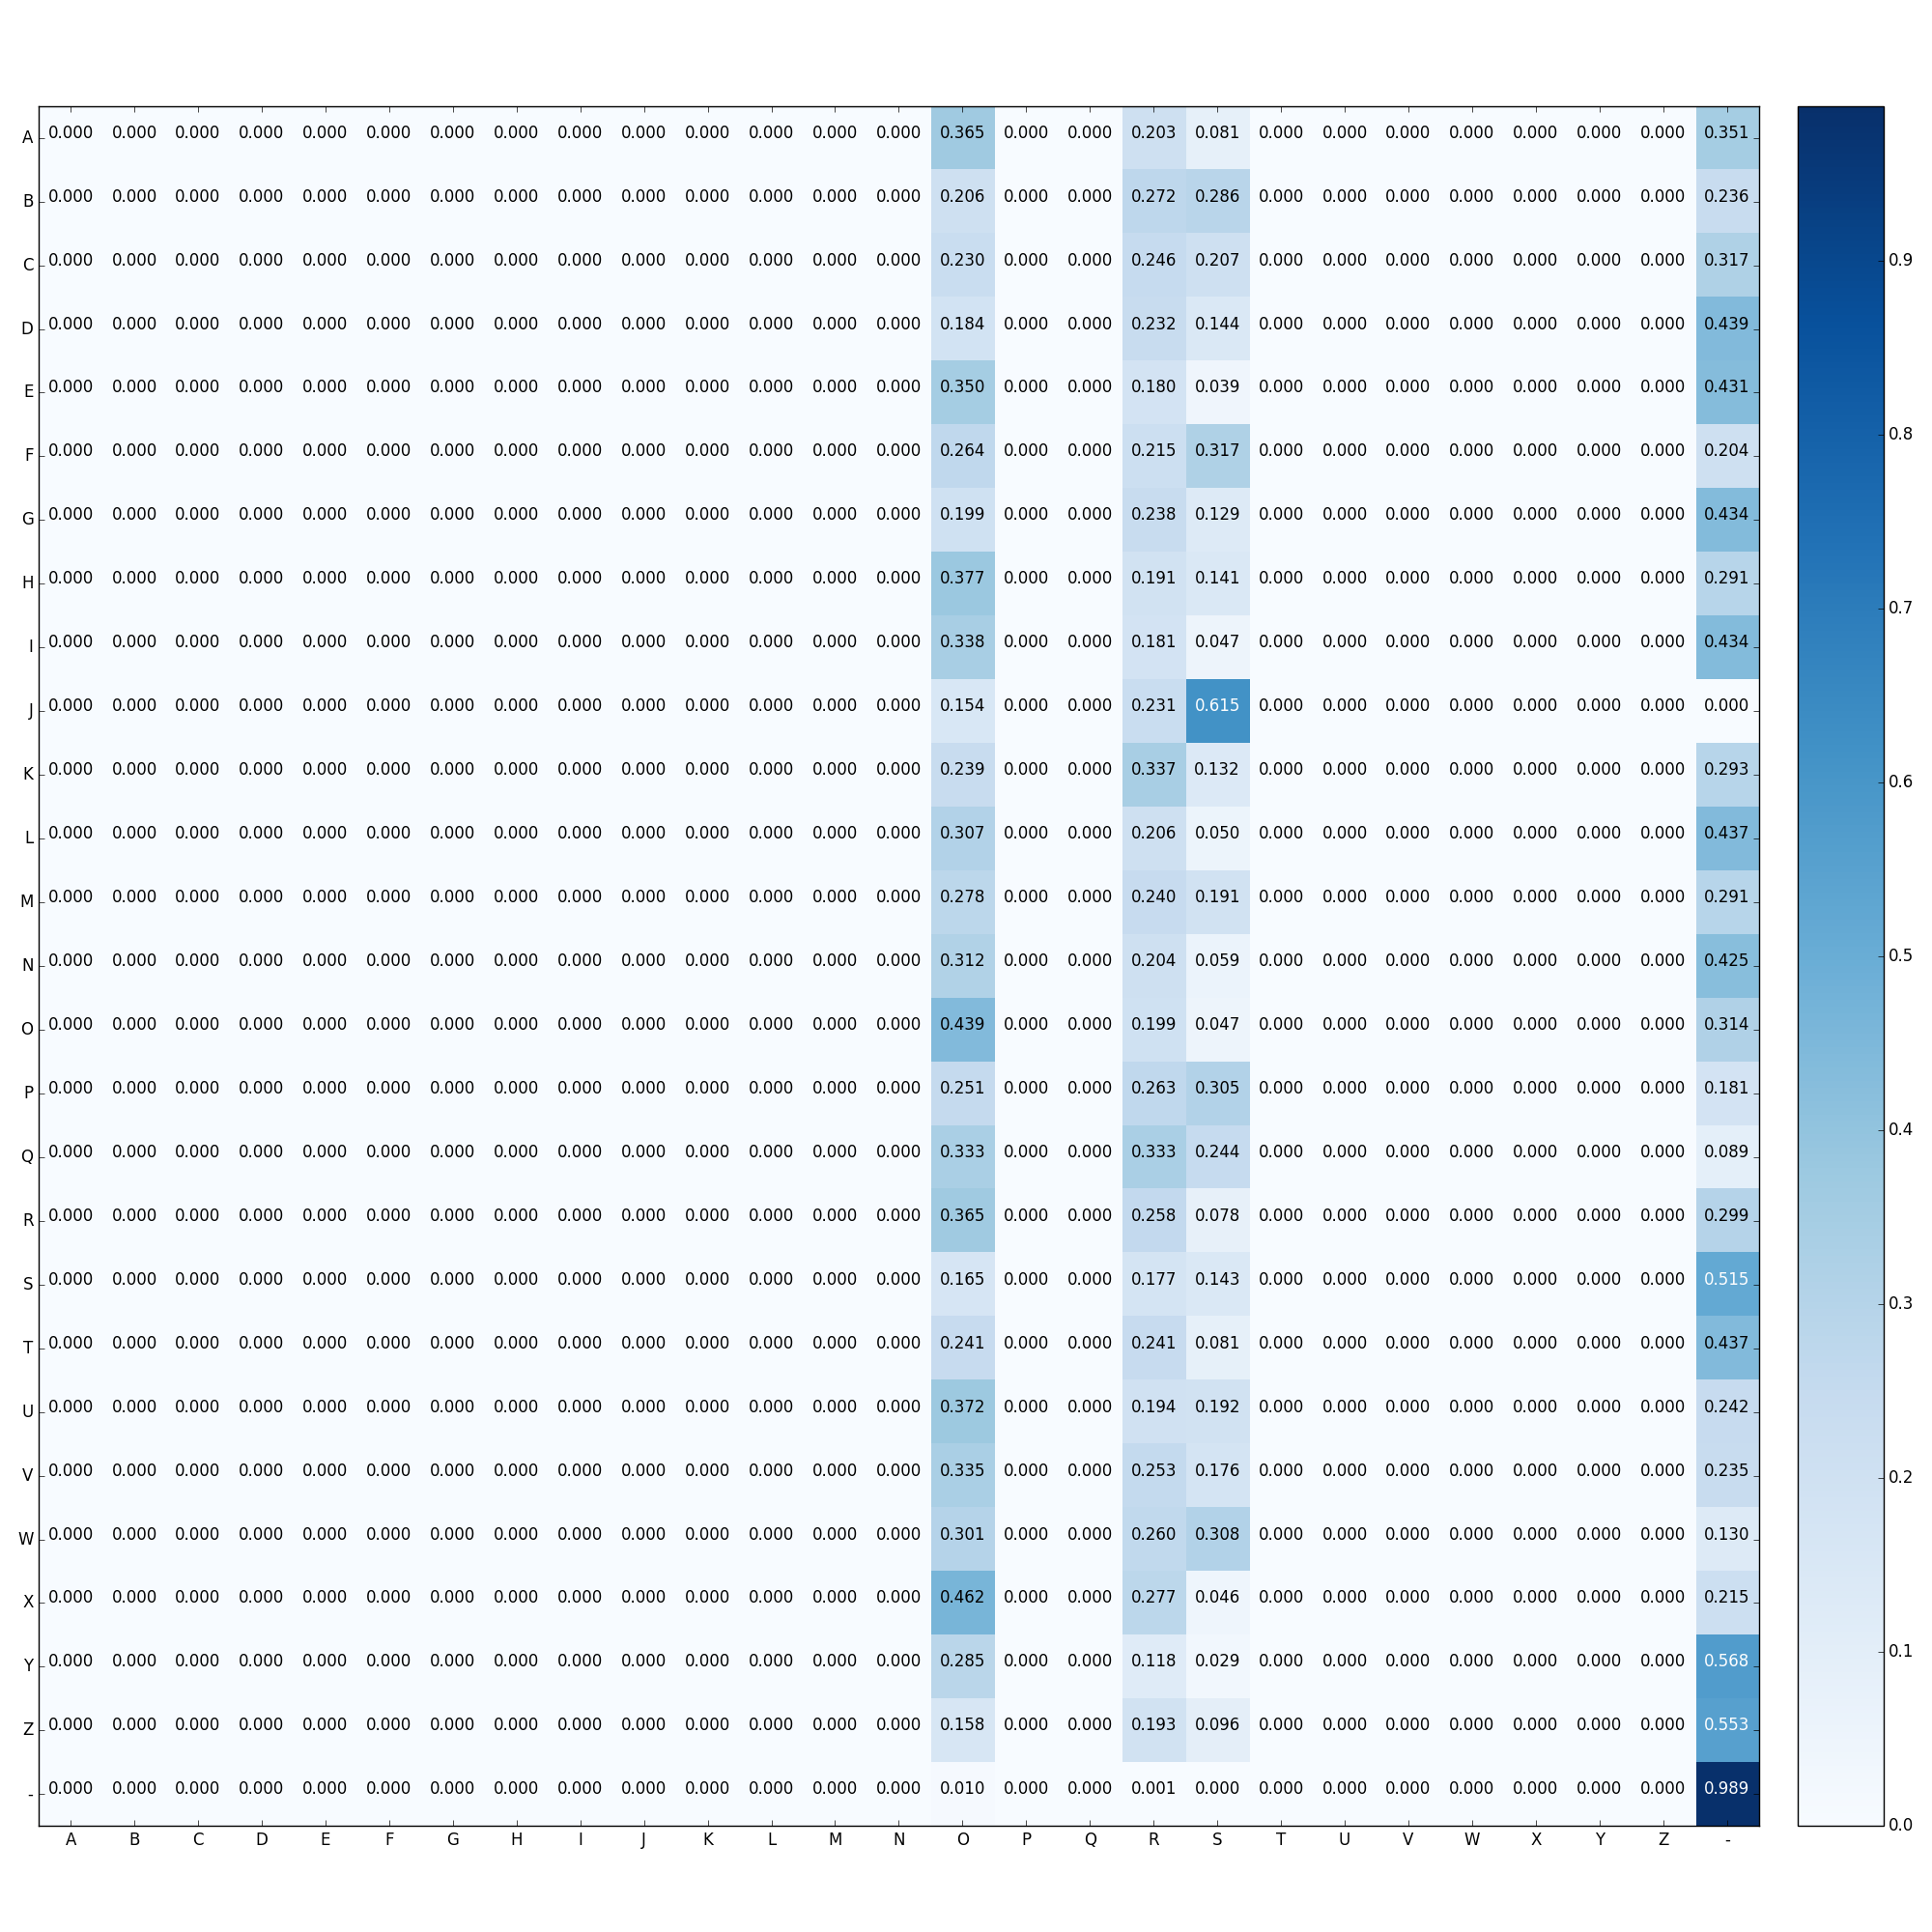
\includegraphics[width=1\textwidth]{fig/results/experiment1/big/vecrep/confusion_matrix.png}
    \caption{Confusion matrix for the best {\tt VecRep} model on the big dataset}
    \label{fig:result1_big_vecrep_confusion_matrix}
\end{figure}

The confusion matrix illustrated in Figure \ref{fig:result1_big_vecrep_confusion_matrix} explains how the {\tt VecRep} model was able to achieve an accuracy of over 50\% on the big dataset. The big dataset had a maximum word length of 20 letters, while most words in the English language, as well as in our datasets, are shorter than this. Shorter words were padded to compensate for the different word-lengths. This padding was done by filling the empty labels with a special padding symbol. The {\tt VecRep} model seem to base its predictions on the most common labels, which would be the padding symbol. It also seems to prefer other common labels such as O, R, and S. Every other cell in the confusion matrix is zero, meaning the model did not predict on more than four of the total 27 classes. The confusion matrix clearly indicates that the {\tt VecRep} model was not able to translate between our two constructed languages. 

\newpage
\subsection{EncDecReg}
\subsubsection{Accuracy and Loss}
\resultplots{fig/results/experiment1/small/encdecreg/}{plot_accuracy.png}{plot_loss.png}{result1_small_encdecreg}{Accuracy and loss for {\tt EncDecReg} on small dataset}{ht}
\resultplots{fig/results/experiment1/medium/encdecreg/}{plot_accuracy.png}{plot_loss.png}{result1_medium_encdecreg}{Accuracy and loss for {\tt EncDecReg} on medium dataset}{hp}
\newpage
\resultplots{fig/results/experiment1/big/encdecreg/}{plot_accuracy.png}{plot_loss.png}{result1_big_encdecreg}{Accuracy and loss for {\tt EncDecReg} on big dataset}{ht}

The plots for the three best {\tt EncDecReg} models indicates that the models were able to learn. The accuracy for all three of them indicates improvement, although the accuracy for the small and medium datasets never improves beyond 60\% accuracy. The loss plots also indicate overfitting, especially on the smallest dataset. The model ran on the biggest dataset seem to improve almost continuously for 400 epochs. This model also had a big spike in the loss values at around epoch 500 but was able to recover after this. These spikes seem to appear with the Adam optimizer when a model is stuck on a plateau, and the average of past squared gradients becomes small, although we are not entirely sure this is the cause.

\newpage
\subsubsection{Confusion Matrix}
\begin{figure}[H]
    \centering
    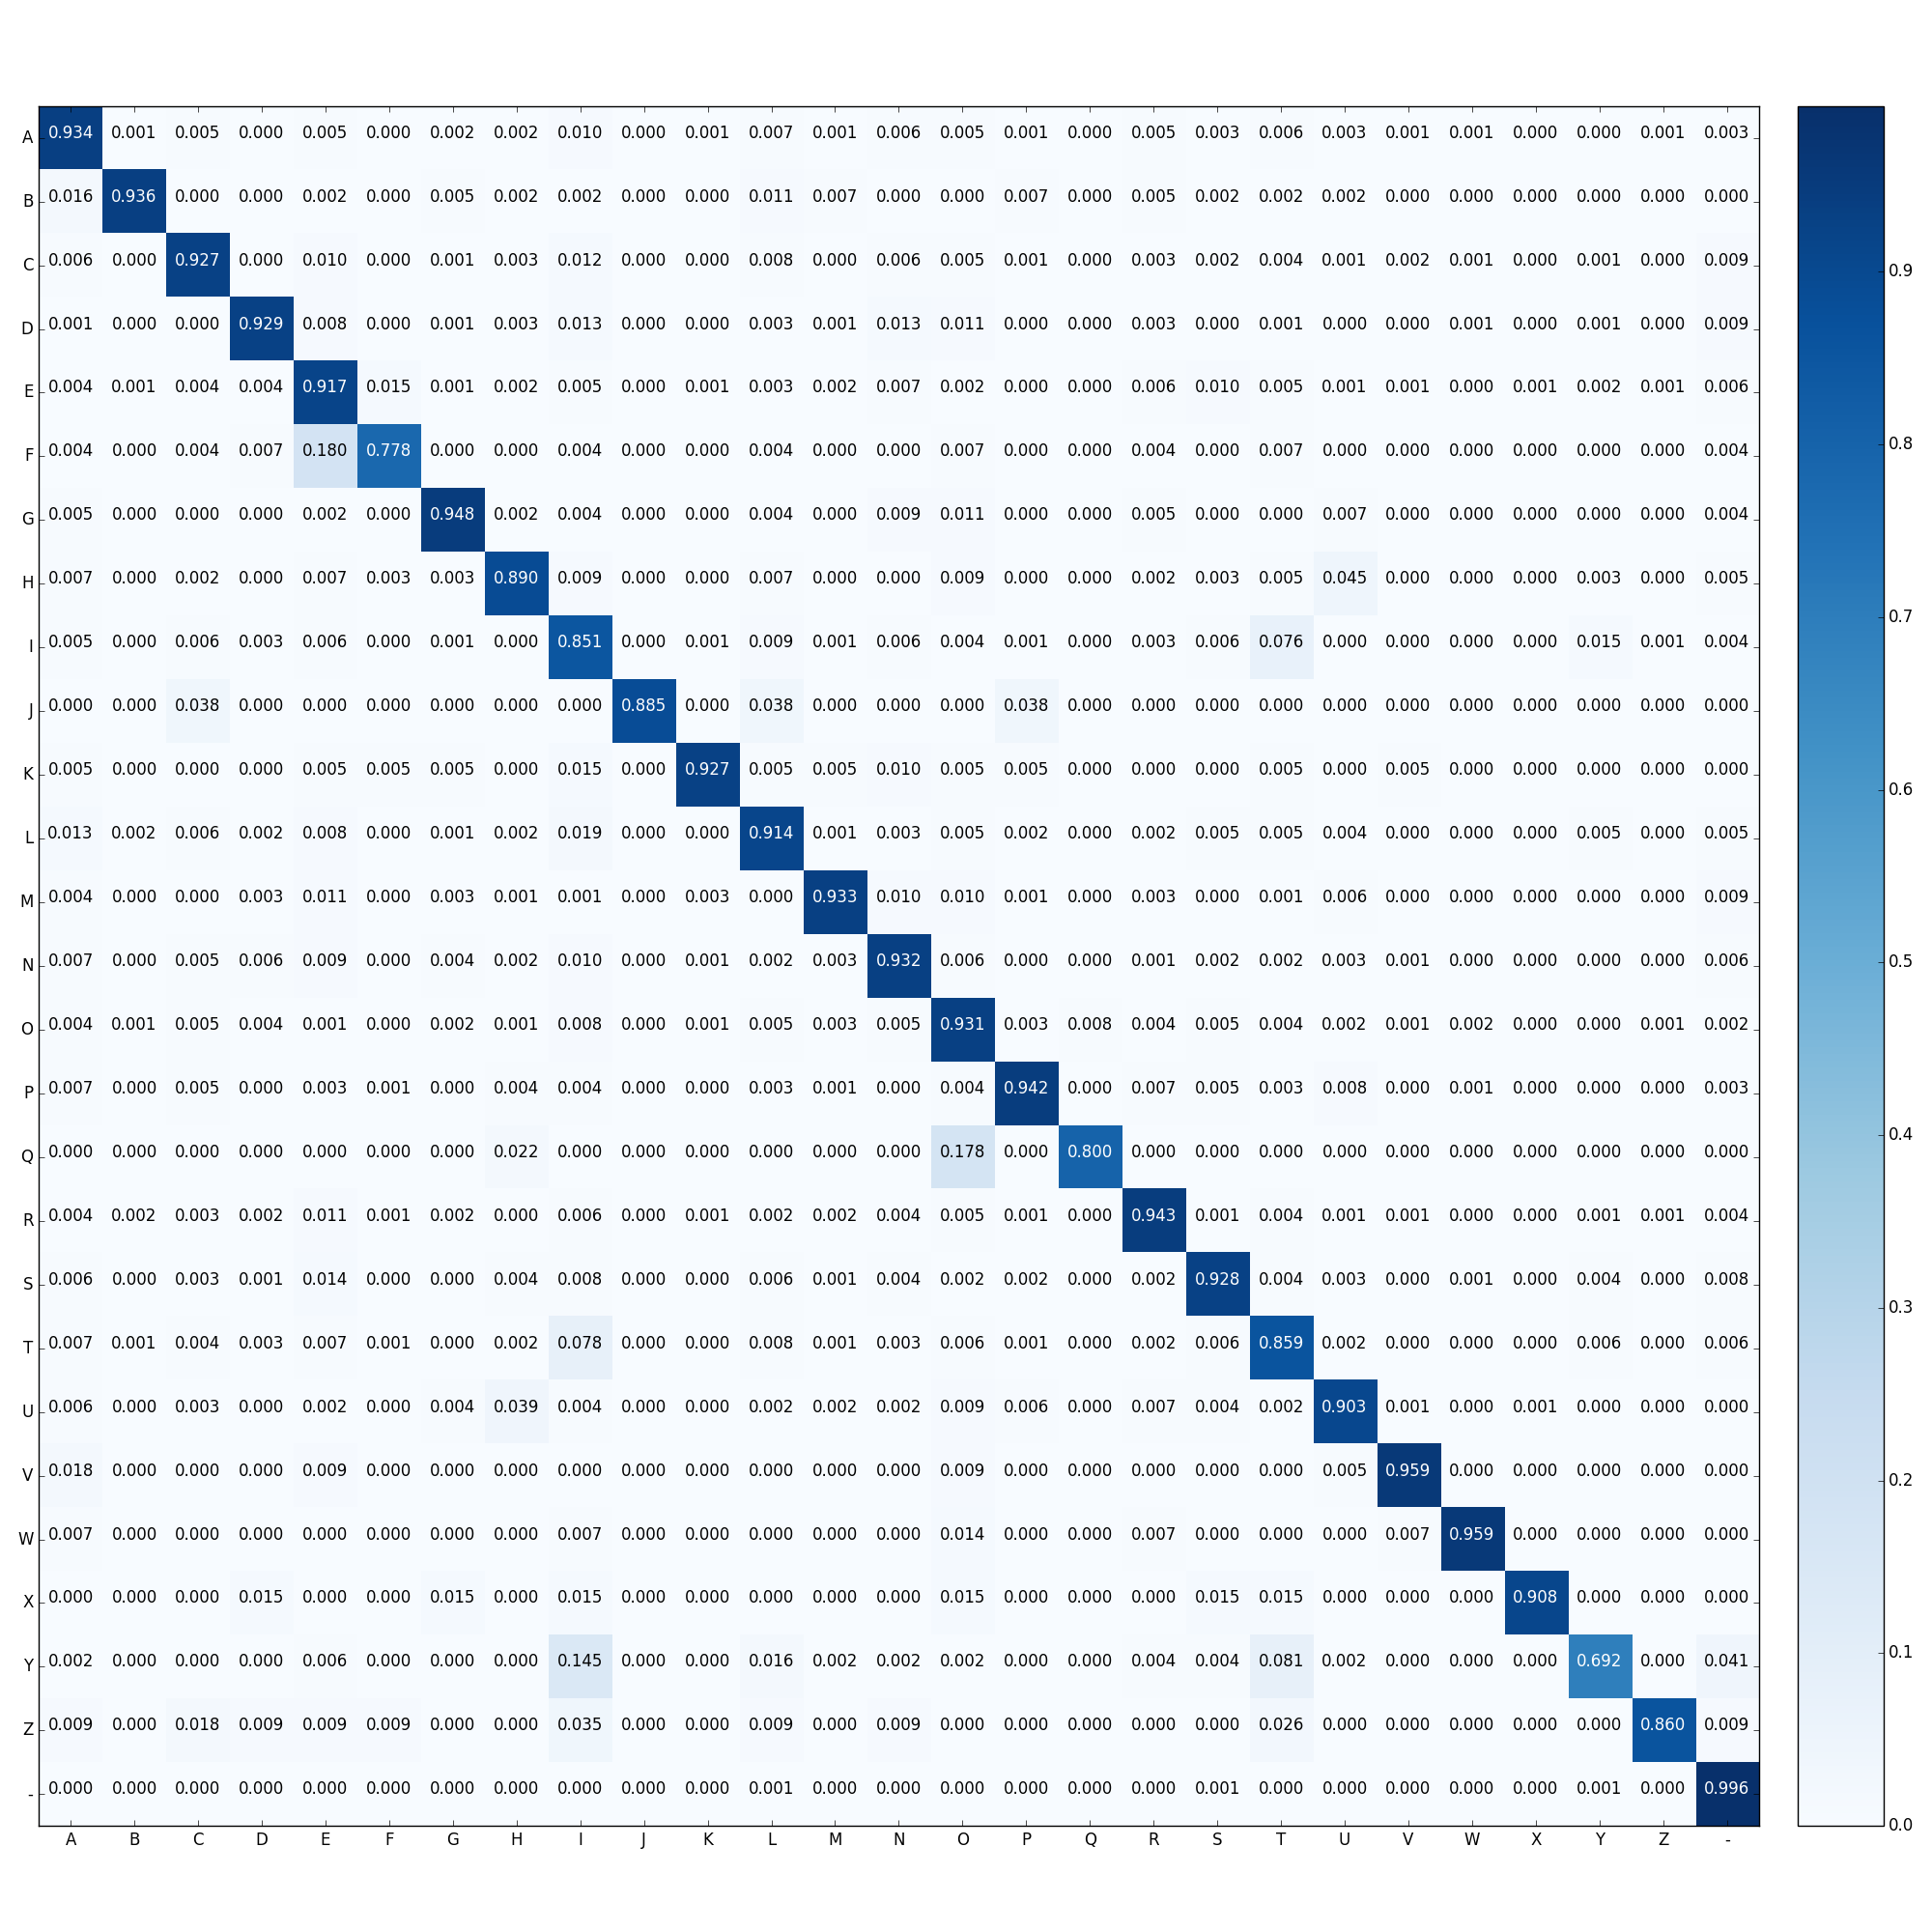
\includegraphics[width=1\textwidth]{fig/results/experiment1/big/encdecreg/confusion_matrix.png}
    \caption{Confusion matrix for the best {\tt EncDecReg} model on the big dataset}
    \label{fig:result1_big_encdecreg_confusion_matrix}
\end{figure}

The {\tt EncDecReg} had an accuracy of almost 95.5\% on the big dataset, which is reflected in the confusion matrix in Figure \ref{fig:result1_big_encdecreg_confusion_matrix}. The confusion matrix has a defined diagonal line with a very high individual accuracy. Most of the labels have an accuracy of over 0.9 with a few exceptions. Y is wrongly labeled as an I in 14.5\% of the instances, and as a T in 8.5\% of the instances. The most wrongly labeled classes are F as an E (18\%) and Q as O (17.8\%).

\newpage
\subsection{EncDecAtt}
\subsubsection{Accuracy and Loss}
\resultplots{fig/results/experiment1/small/encdecatt/}{plot_accuracy.png}{plot_loss.png}{result1_small_encdecatt}{Accuracy and loss for {\tt EncDecAtt} on small dataset}{ht}
\resultplots{fig/results/experiment1/medium/encdecatt/}{plot_accuracy.png}{plot_loss.png}{result1_medium_encdecatt}{Accuracy and loss for {\tt EncDecAtt} on medium dataset}{hp}
\newpage
\resultplots{fig/results/experiment1/big/encdecatt/}{plot_accuracy.png}{plot_loss.png}{result1_big_encdecatt}{Accuracy and loss for {\tt EncDecAtt} on big dataset}{ht}

These plots show much of the same as the plots for the {\tt EncDecReg} model. The overfitting is less apparent than with the {\tt EncDecReg} model, although the {\tt EncDecAtt} model also seems to overfit on both the small and medium datasets. The model for the big dataset also has multiple spikes, similar to the {\tt EncDecReg} model. This model also seems to improve for many epochs on the biggest dataset.

\newpage
\subsubsection{Confusion Matrix}
\begin{figure}[H]
    \centering
    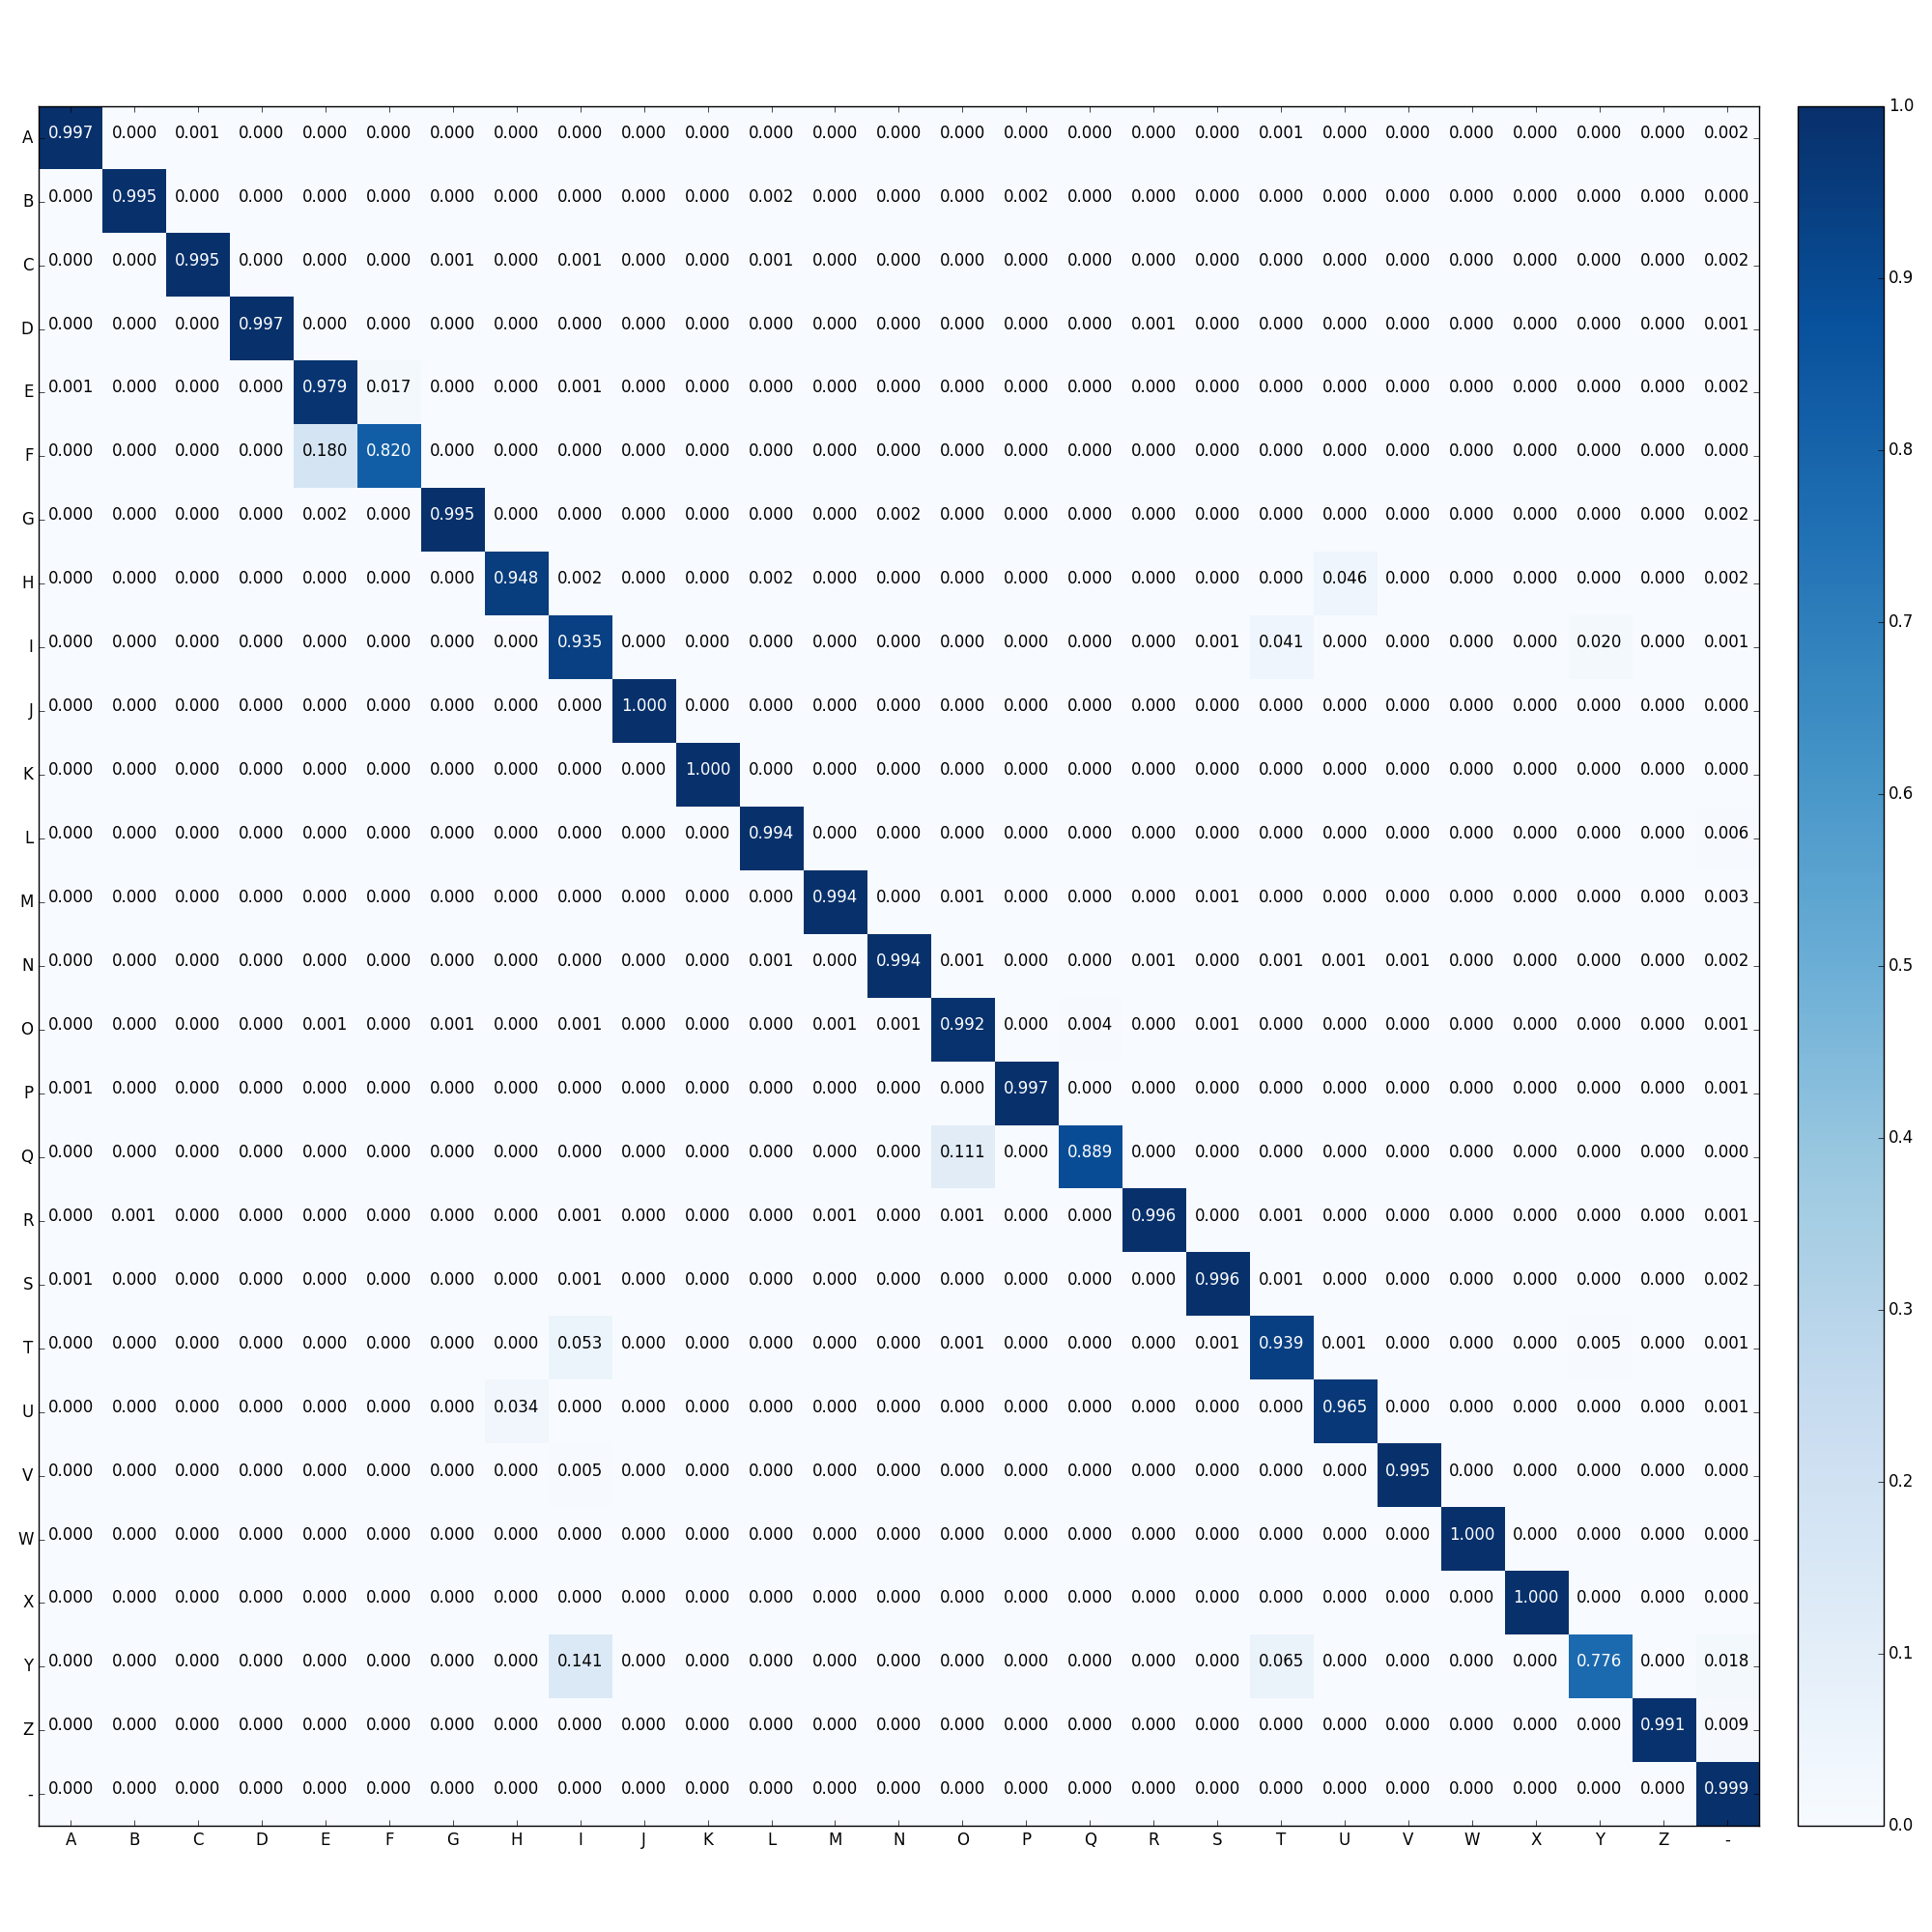
\includegraphics[width=1\textwidth]{fig/results/experiment1/big/encdecatt/confusion_matrix.png}
    \caption{Confusion matrix for the best {\tt EncDecAtt} model on the big dataset}
    \label{fig:result1_big_encdecatt_confusion_matrix}
\end{figure}

The confusion matrix for the {\tt EncDecAtt} model (Figure \ref{fig:result1_big_encdecatt_confusion_matrix}) has high individual accuracy, similar to the results of the {\tt EncDegReg} model, although this model has improved even further. The {\tt EncDegAtt} model successfully classifies four classes without a single error, and only three classes have a lower accuracy than 0.9. However, also this model seem to struggle with some of the same misclassifications as the {\tt EncDegReg} model, namely F as E, Q as O, and Y as I or T.

%%=========================================

\section{Handling of Two Fonts}
\label{sec:handling_of_two_fonts}
Table \ref{table:accuracy_two_fonts} contains the results for each model on the dataset with two fonts. As seen in this table, the accuracy of the {\tt EncDecAtt} is more or less unaffected by the introduction of a second font, whereas the {\tt EncDecReg} and {\tt VecRep} models have reduced accuracy compared to previous experiments. 

\begin{table}[H]
    \centering
    \begin{tabular}{|l|l|}
        \hline 
        \textbf{Model}                  & \textbf{Accuracy}         \\ \hline
        {\tt VecRep }                   & 40.49\%                   \\ \hline
        {\tt EncDecReg}                 & 88.21\%                   \\ \hline
        {\tt EncDecAtt}                 & 98.93\%                   \\ \hline
    \end{tabular}
    \caption{Accuracy for each model on a dataset with two fonts}
    \label{table:accuracy_two_fonts}
\end{table}

\subsection{Accuracy and Loss for Each Model}
\resultplots{fig/results/experiment2/vecrep/}{plot_accuracy.png}{plot_loss.png}{result2_vecrep}{Accuracy and loss for {\tt VecRep} handling two fonts}{ht}
\resultplots{fig/results/experiment2/encdecreg/}{plot_accuracy.png}{plot_loss.png}{result2_encdecreg}{Accuracy and loss for {\tt EncDecReg} handling two fonts}{hp}
\newpage
\resultplots{fig/results/experiment2/encdecatt/}{plot_accuracy.png}{plot_loss.png}{result2_encdecatt}{Accuracy and loss for {\tt EncDecAtt} handling two fonts}{ht}

Again the loss plot for the {\tt VecRep} indicates that this model is unable to learn properly, and the loss value seems to worsen after a few couple of epochs. Both the encoder-decoder models seem to overfit, although the {\tt EncDecReg} model overfits significantly after about 130 epochs.

%%=========================================

\newpage
\section{Noise Handling}
\label{sec:noise_handling}
Table \ref{table:noise_accuracy} contains the accuracy of the {\tt EncDegAtt} model as the amount of noise was increased. The ``Noise alterations,'' e.i. the actual amount of bits altered from a correct 1 to an incorrect 0, or vice versa, is also listed. 

\begin{table}[ht]
    \centering
    \begin{tabular}{|l|l|l|}
        \hline 
        \textbf{Noise factor}          & \textbf{Noise alterations}       & \textbf{Accuracy}         \\ \hline
        0\%                            & 0\%                              & 98.06\%                   \\ \hline
        2\%                            & 1.49\%                           & 95.83\%                   \\ \hline
        5\%                            & 2.98\%                           & 93.35\%                   \\ \hline
        6\%                            & 3.46\%                           & 91.40\%                   \\ \hline
        8\%                            & 4.45\%                           & 90.93\%                   \\ \hline
        9\%                            & 4.96\%                           & 72.25\%                   \\ \hline
        10\%                           & 5.46\%                           & 69.36\%                   \\ \hline
        15\%                           & 7.94\%                           & 66.77\%                   \\ \hline
        20\%                           & 10.41\%                          & 59.51\%                   \\ \hline
        40\%                           & 20.32\%                          & 47.67\%                   \\ \hline
        50\%                           & 25.28\%                          & 46.20\%                   \\ \hline
        60\%                           & 30.18\%                          & 45.29\%                   \\ \hline
    \end{tabular}
    \caption{Accuracy for the {\tt EncDecAtt} model}
    \label{table:noise_accuracy}
\end{table}

\begin{figure}[ht]
    \centering
    \captionsetup{justification=centering}
    \begin{tikzpicture}
        \begin{axis}[
            xmin=0, xmax=60,
            ymin=0, ymax=1,
            minor y tick num={5},
            minor x tick num={1},
            ylabel=accuracy,
            xlabel=noise,
        ]
            \addplot[draw=red] table[x index=0,y index=1,col sep=comma]{data/noise.csv};
        \end{axis}%
    \end{tikzpicture}%
    \caption{Change of accuracy as the amount of noise is increased}
    \label{fig:noise_accuracy}
\end{figure}

The accuracy is also plotted in Figure \ref{fig:noise_accuracy}, which illustrates how the accuracy deteriorates as the amount of noise was increased. This graph illustrates how the deterioration of the accuracy first falls fast, then flattens out once the amount of noise gets more and more dominant. As shown in both the table and the graph, the accuracy decreased by less than 1.5\% when the noise was increased from 40\% to 50\%. Similarly, the accuracy decreased with less than a percent when the noise rose to 60\%. This is in contrast to how the accuracy decreased by almost 5\% when the noise was introduced to a perfect dataset, compared to a dataset with 5\% noise. Further, the accuracy decreased by 24\% when the noise was increased from 5\% to 10\%.

This shows the difference in accuracy when learning and predicting on datasets that are perfect, near-perfect, and datasets with significant amounts of noise. It also shows that increasing noise on datasets that already have much noise in them have a smaller effect on the accuracy.

%%=========================================

\section{Stress Test}
\label{sec:stress_test}
This experiment was carried out on the models {\tt EncDecReg} and {\tt EncDecAtt}, as the {\tt VecRep} model already had poor results on the experiments that were significantly simpler. The results are presented in Table \ref{table:accuracy_stress_test}.

\begin{table}[ht]
    \centering
    \begin{tabular}{|l|l|}
        \hline 
        \textbf{Model}                  & \textbf{Accuracy}         \\ \hline
        {\tt EncDecReg}                 & 55.02\%                   \\ \hline
        {\tt EncDecAtt}                 & 88.44\%                   \\ \hline
    \end{tabular}
    \caption{Accuracy for each model on the stress test}
    \label{table:accuracy_stress_test}
\end{table}

\newpage
\subsection{EncDecReg Results}
\begin{figure}[ht]
    \centering
    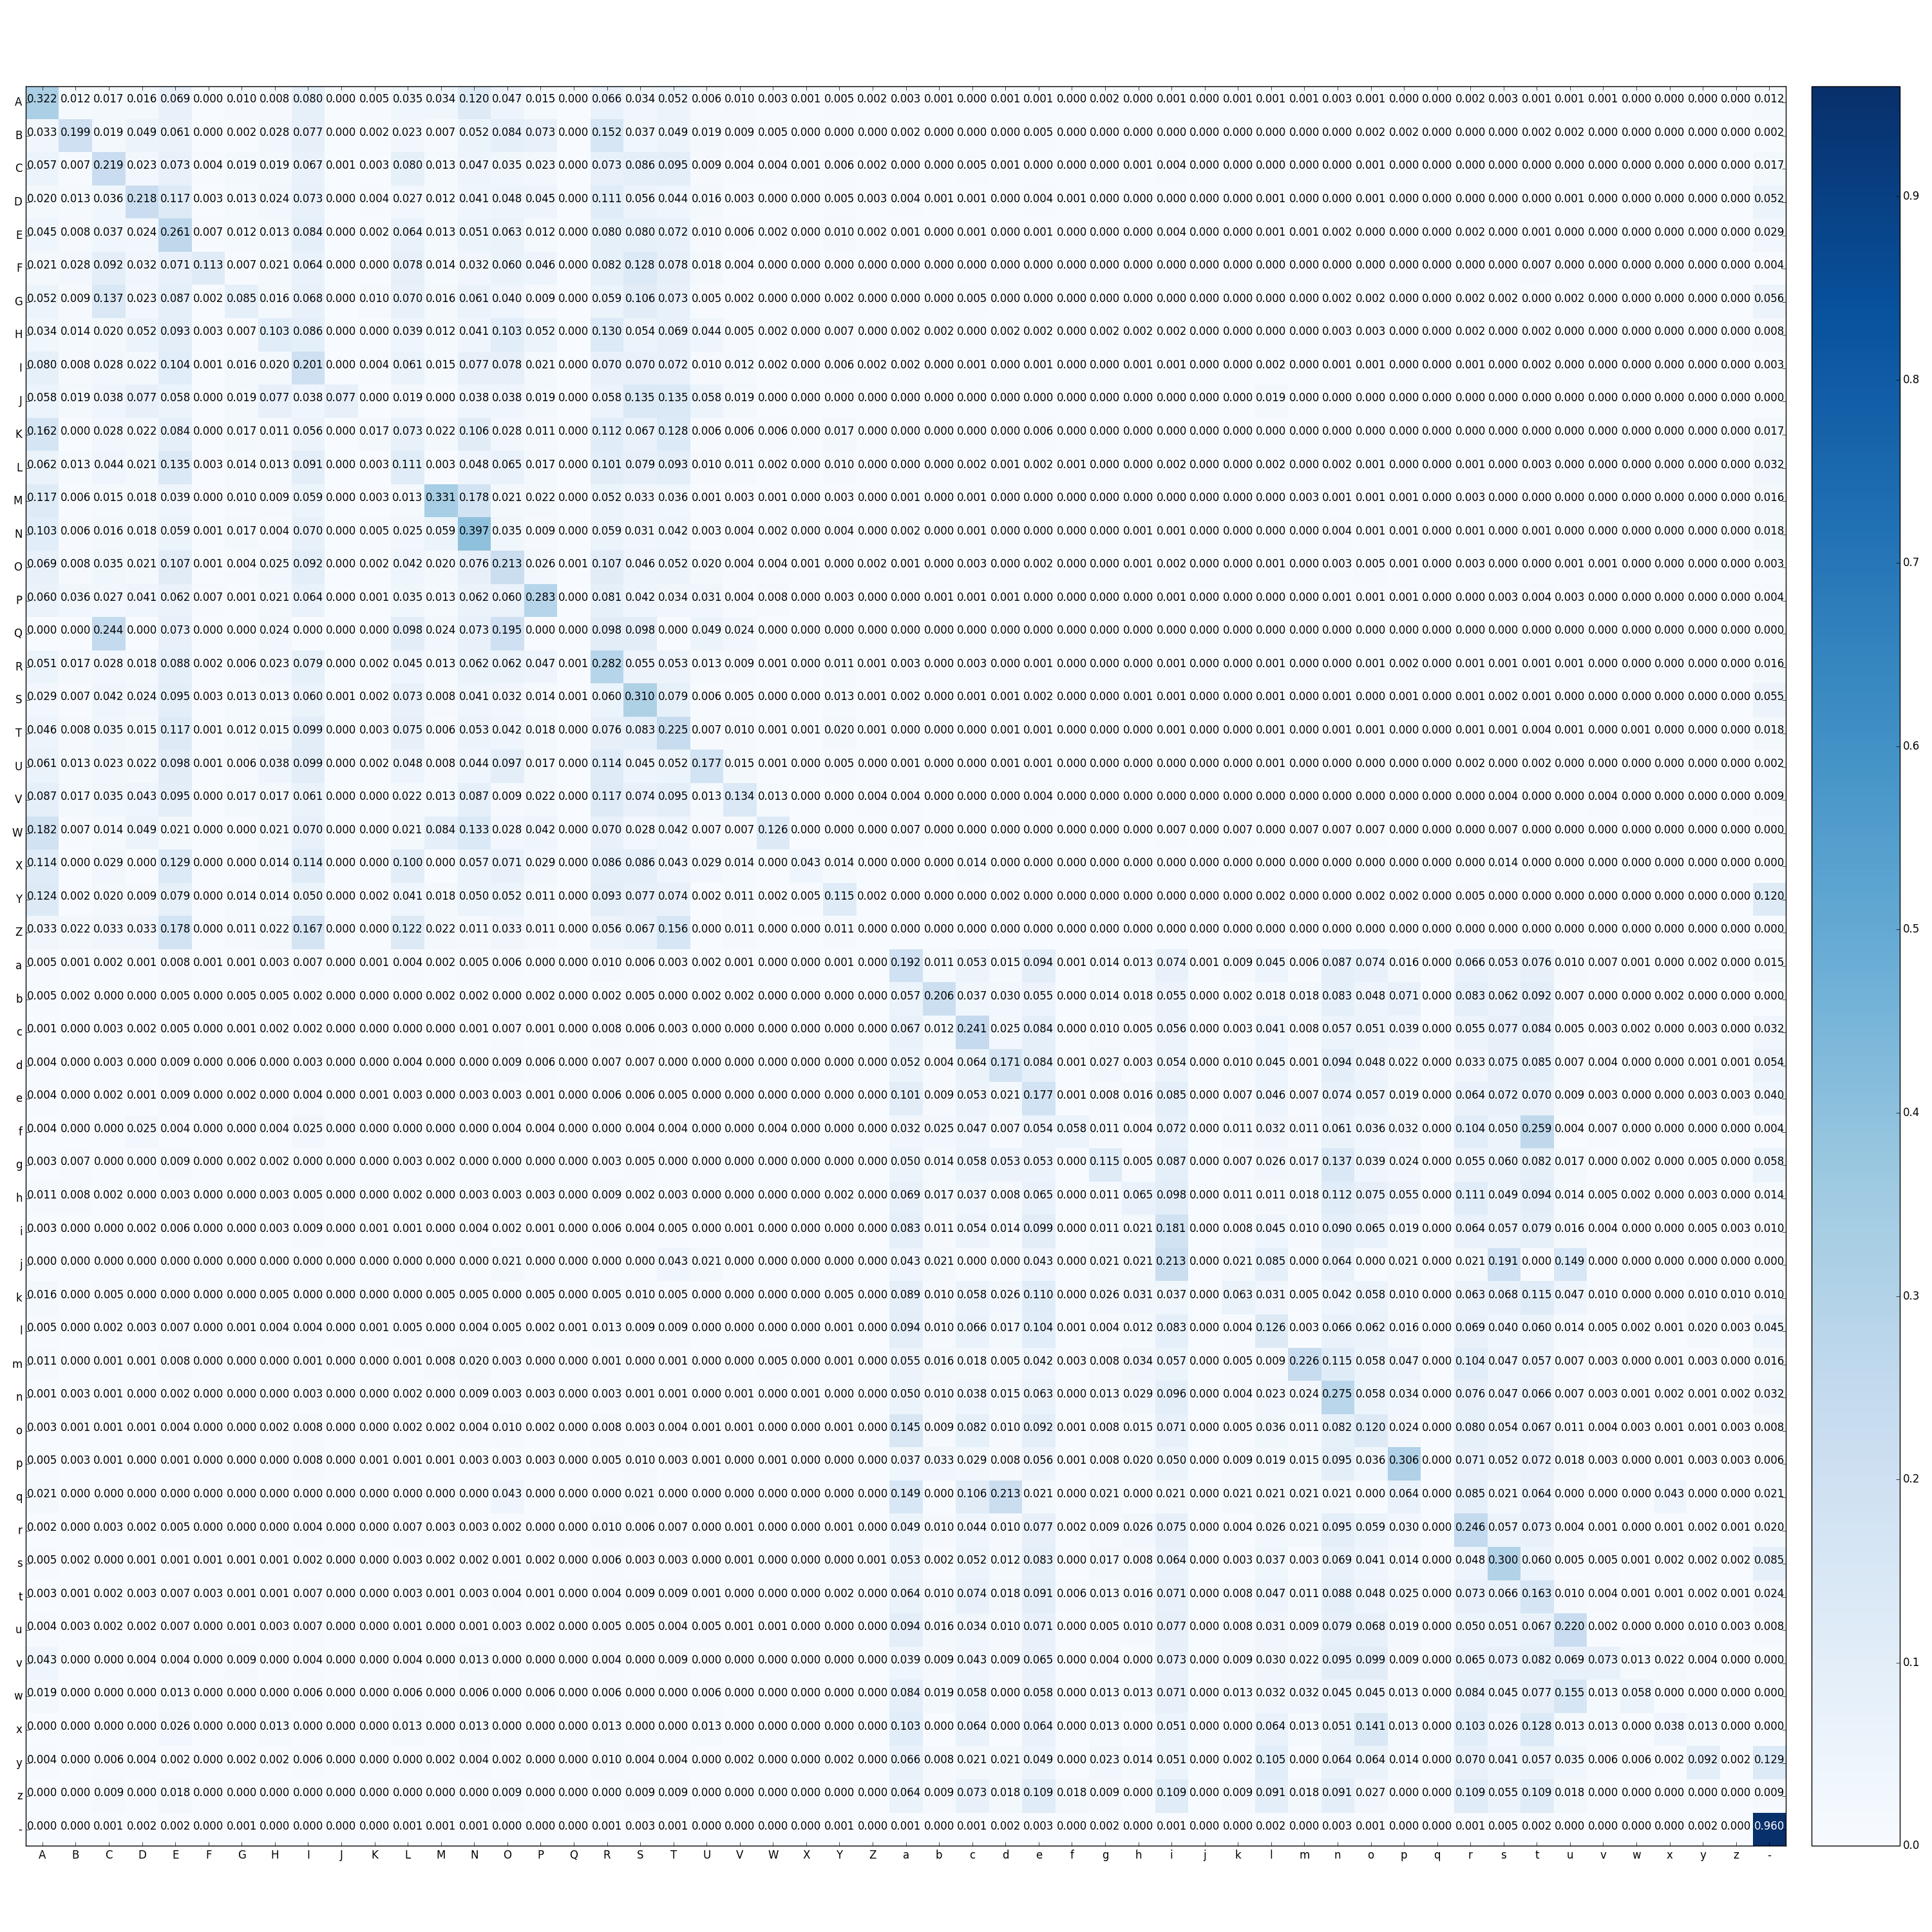
\includegraphics[width=1\textwidth]{fig/results/experiment4/encdecreg/confusion_matrix.png}
    \caption{Confusion matrix for the best {\tt EncDecReg} model on the stress test}
    \label{fig:result4_encdecreg_confusion_matrix}
\end{figure}

Shown in Figure \ref{fig:result4_encdecreg_confusion_matrix} is the confusion matrix for the best {\tt EncDecReg} model on the stress test. As depicted in this matrix, the model had a hard time classifying the labels correctly, which corresponds to its accuracy of 55\%. However, the confusion matrix shows traces of a faint diagonal line going from corner-to-corner, indicating correct classifications. In general, the model seems capable of separating the upper-cased and lower-cased letters from each other, having almost no incorrect classifications shared between the two halves of the matrix. For both groups of upper-cased and lower-cased letters, the model seems to favor a few letters in each, wrongly classifying them across a wide spectrum of other letters.

\newpage
\subsection{EncDecAtt Results}
\begin{figure}[ht]
    \centering
    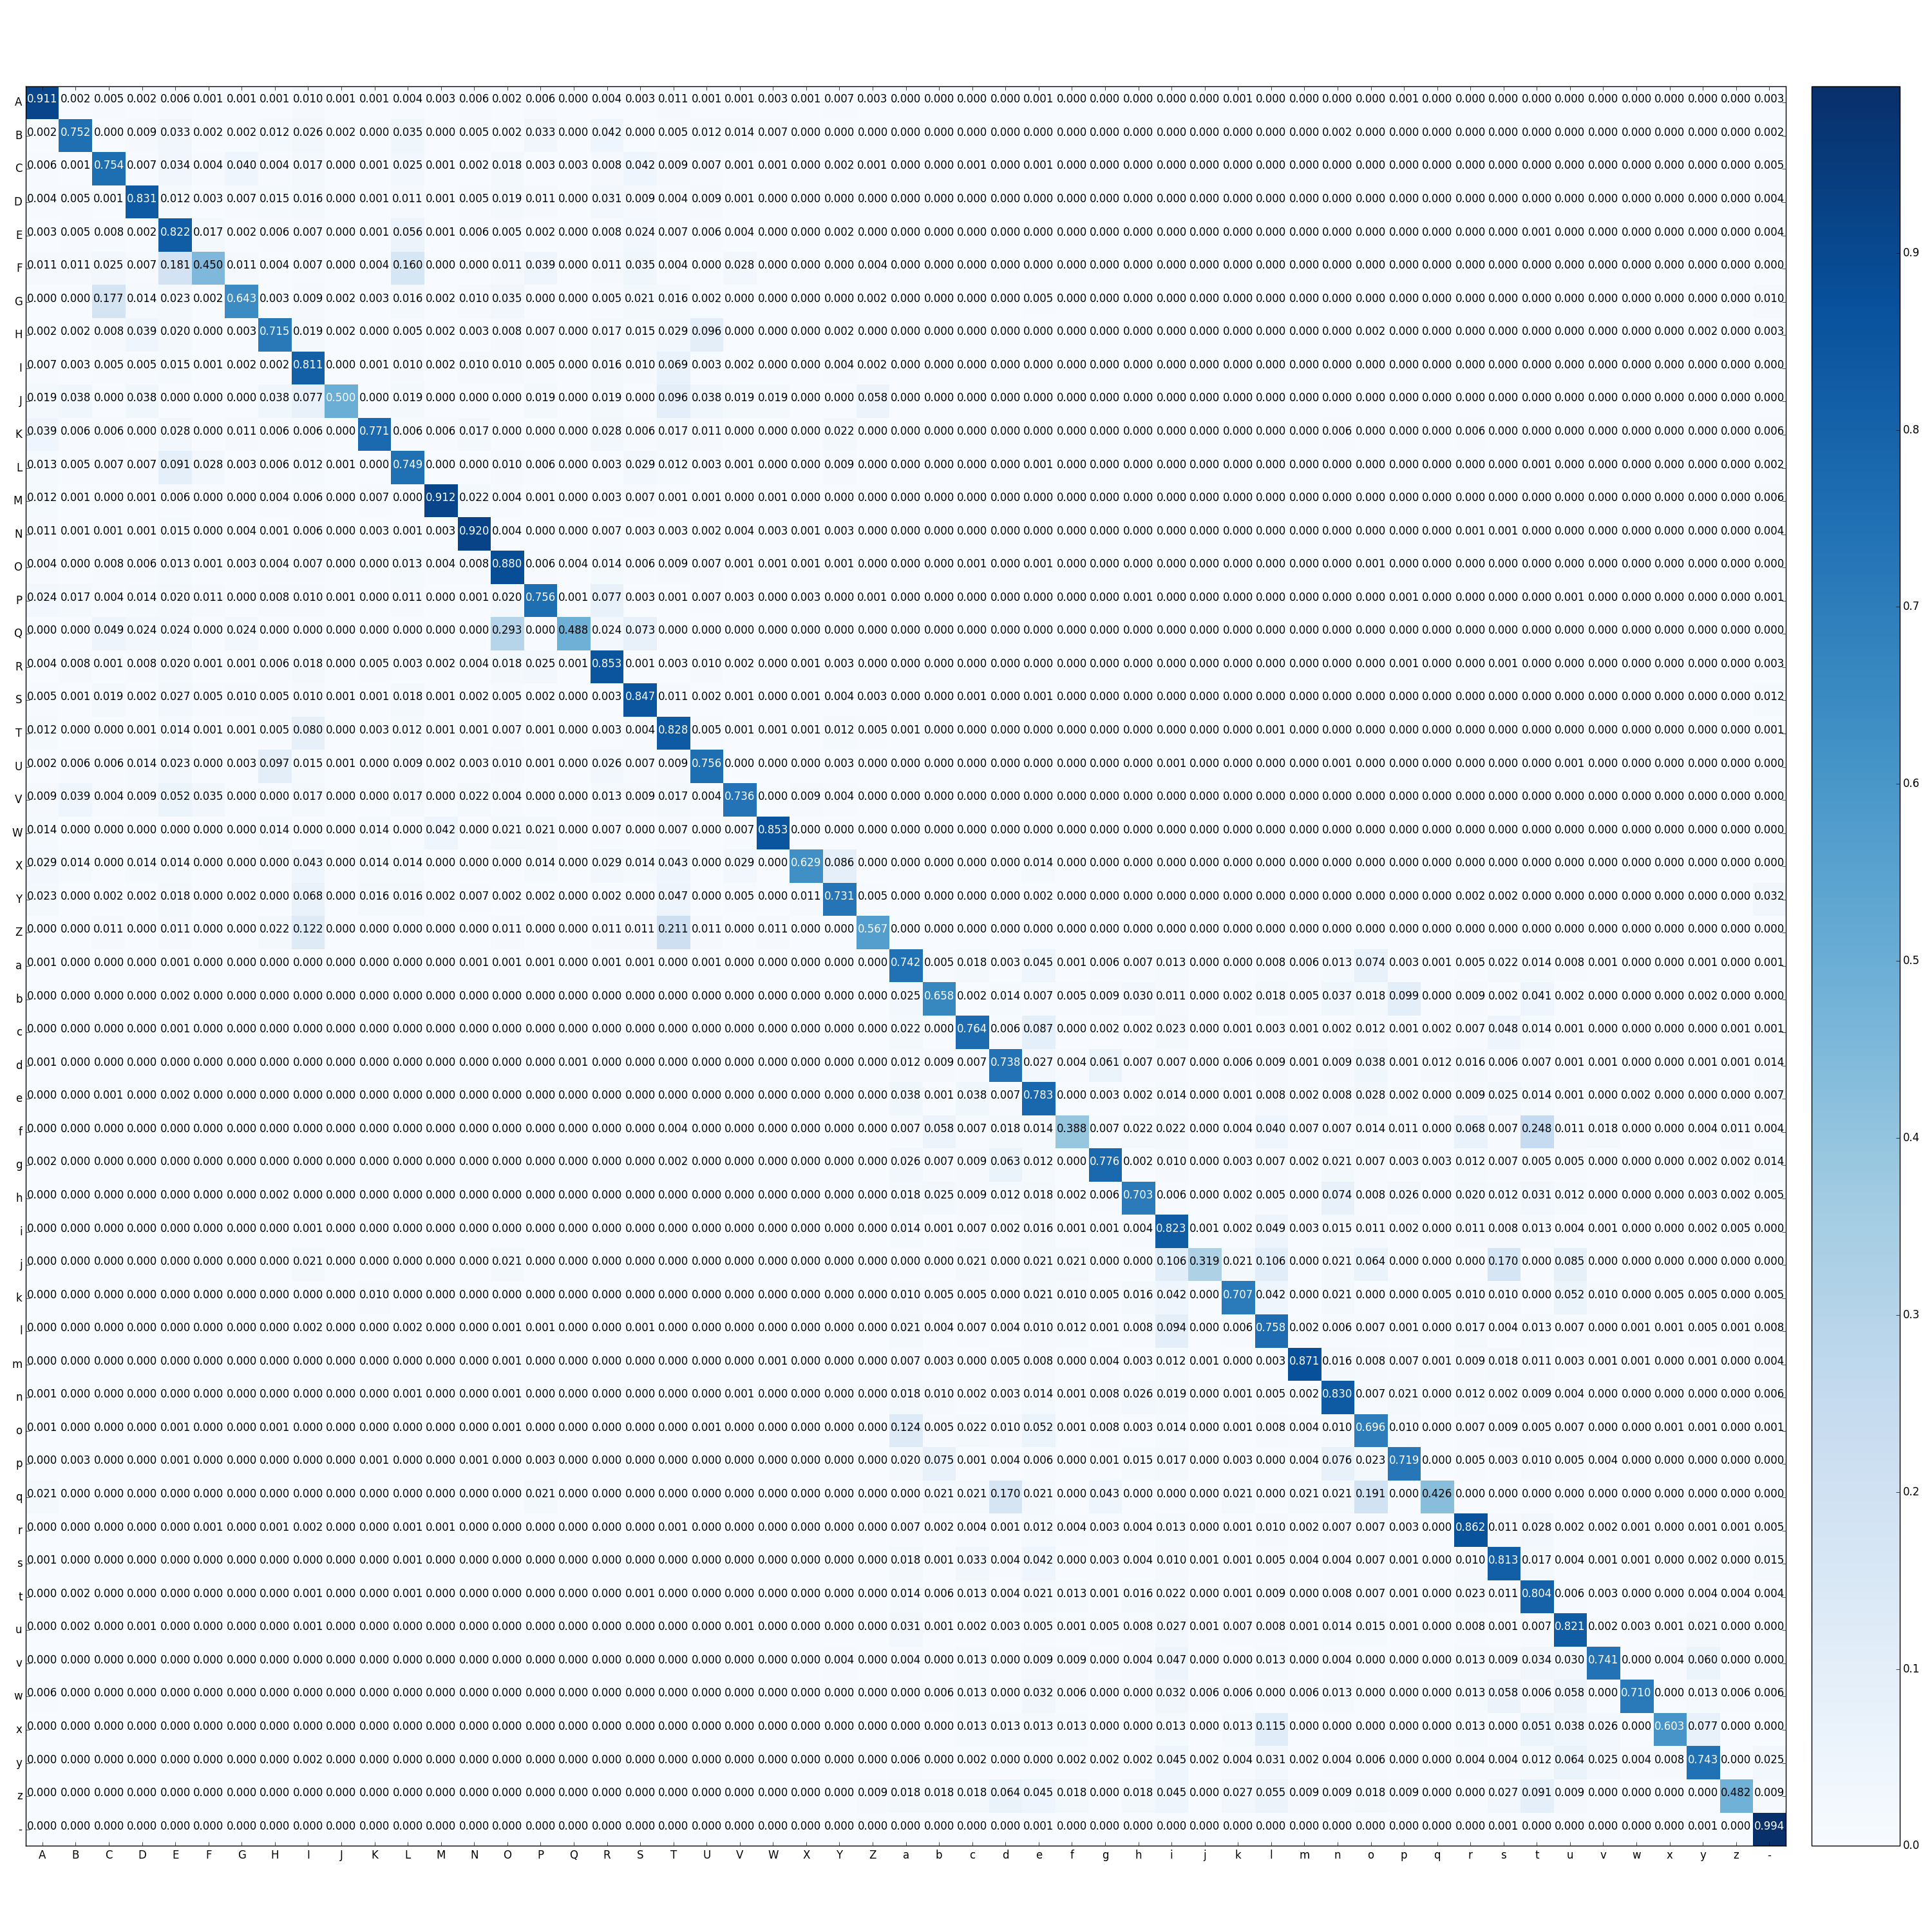
\includegraphics[width=1\textwidth]{fig/results/experiment4/encdecatt/confusion_matrix.png}
    \caption{Confusion matrix for the best {\tt EncDecAtt} model on the stress test}
    \label{fig:result4_encdecatt_confusion_matrix}
\end{figure}

Figure \ref{fig:result4_encdecatt_confusion_matrix} shows the classification matrix of the best {\tt EncDecAtt} model on the stress test. This matrix depicts a clear diagonal line from corner-to-corner, indicating that the model has been able to, for the most part, classifying labels correctly. Although there are certain labels that are misclassified, the vast majority of the labels are correctly classified, which corresponds to the accuracy of over 88\% for this model. The confusion matrix also shows almost no overlap between the labels in the upper-cased and lower-cased classes, indicating that also this model was able to separate these groups from each other. Some of the labels are repeatably misclassified, and many of these are the same misclassifications we have seen in other tests for the same model.

%%=========================================

\section{Result Discussion}
\label{sec:result_discussion}
In this section, we discuss and compare the various results and models against each other. We also answer the research questions we defined earlier and discuss our results in the context of our research goal.

\subsection{General Discussion}
The first experiment indicated that the {\tt VecRep} model was unable to learn the problem to a satisfactory degree. The confusion matrix indicates that the model is unable to translate anything, and relies on classifying the padded values. {\tt EncDecReg} and {\tt EncDecAtt} both show indications that they learned to translate between our two languages, especially when the size of the datasets was increased. The {\tt EncDecAtt} model outperformed the {\tt EncDecReg} model in every single experiment. The latter model also reached impressive results for the most complicated experiments we carried out. While the only difference between these two encoder-decoder based models is the attention mechanism, there is a big difference in their performance. We see this both when the datasets are small, and in more complex experiments.

\subsection{Research Questions}

\subsubsection{Ambiguity in Character Signature Sequences}
In our first research question, \textbf{RQ1}, we asked if the models were able to deal with ambiguity in the input data. In our first experiment, we used the same system configurations as shown in Table \ref{table:signature_sequence_example}, which we used to illustrate how some of the letter signatures were either identical or subsequences of another signature. In this table, we showed that the letters C, I, J, L, T, and Y all shared the same unique signature of three black pixels. The other letters that also shared identical signatures were E and F, H and U, O and Q, and S and X. 

Comparing these sets to the confusion matrices, we can see that some of these characters were indeed those the models struggled to classify correctly. Specifically, U, I and T, F and E, as well as Q and O were problematic for both the encoder-decoder models, although their accuracy was no lower than 0.692 for the {\tt EncDegReg} model, and 0.776 for the {\tt EncDegAtt} model on any of these labels. The most commonly wrongly classified label was an E as F, with both the models having an equal confusion of 0.18. 

These numbers indicate that there is still room for improvement, and that ambiguity may be a concern. Nevertheless, we have concluded that in the context of our experiments and results, the models were able to handle ambiguity to a degree we found satisfactory.

\newpage
\subsubsection{Handling of Multiple Fonts}
Experiments have indicated that both the encoder-decoder models were able to handle more than one font, as questioned in \textbf{RQ2}. The model without the attention mechanism had visibly lower accuracy than experiments carried out on datasets consisting of one font. The {\tt EncDecAtt} model was more or less unaffected by the introduction of an additional font in the second experiment. The same model also yielded good results in the stress test, where the input consisted of five different fonts. On the same test, the {\tt EncDecReg} model had lower accuracy, indicating that this model may be unsuitable for input with such high variance in the sequences.

\subsubsection{Handling of Noise}
Lastly, \textbf{RQ3} asked if the model(s) were able to adapt to noise and imperfect input data. Experiments have shown that the {\tt EncDecAtt} model was able to handle increasing amounts of noise, although the accuracy decreased as the noise factor increased. For a noise factor of 5\%, the accuracy decreased by a little less than 5\%, while a noise factor of 10\% decreased the accuracy by more than 28\%. As there is no real answer to how much noise a model should handle, or how robust a model should be to noise, there is no way to define a hard threshold between reasonable amounts of noise, and excessive amounts of noise. We have decided to conclude this question by stating that the {\tt EncDecAtt} model was able to handle noise in a satisfactory manner. 

\subsection{Discussing the Research Goal}
Our goal in this thesis was to create a model that was able to use signature sequences to recognize letters and words. The results from our experiments, which has been presented in this chapter, indicates that we were successful in reaching this goal. The two encoder-decoder models, especially the {\tt EncDecAtt} model, has been successful in recognizing words with a high accuracy, and we have found these results satisfactory for our evaluation.

%%=========================================

\section{Analysis}
\label{sec:reasoning}
In this section, we look closer at how the encoder-decoder models work, and we analyze the models in the context of our results. The goal of this analysis is to investigate the cause and the affect for various parts of the encoder-decoder framework.

\subsection{Encoding}
We first look at the encoding mechanism of the encoder-decoder framework and how it works. We do this by training a model on a dataset with 1\% noise and then feeding the same words multiple times with the same amount of noise, but different random seeds. We fed the model three words one thousand times each and plotted the encoded context vector in a low dimensional space using t-distributed Stochastic Neighbor Embedding (t-SNE). t-SNE is a tool for visualizing high-dimensional data. It converts similarities between data points to joint probabilities and tries to minimize the Kullback-Leibler divergence between the joint probability distribution between low-dimensional and high-dimensional data \citep{maaten2008visualizing}.

\begin{figure}[!ht]
    \centering
    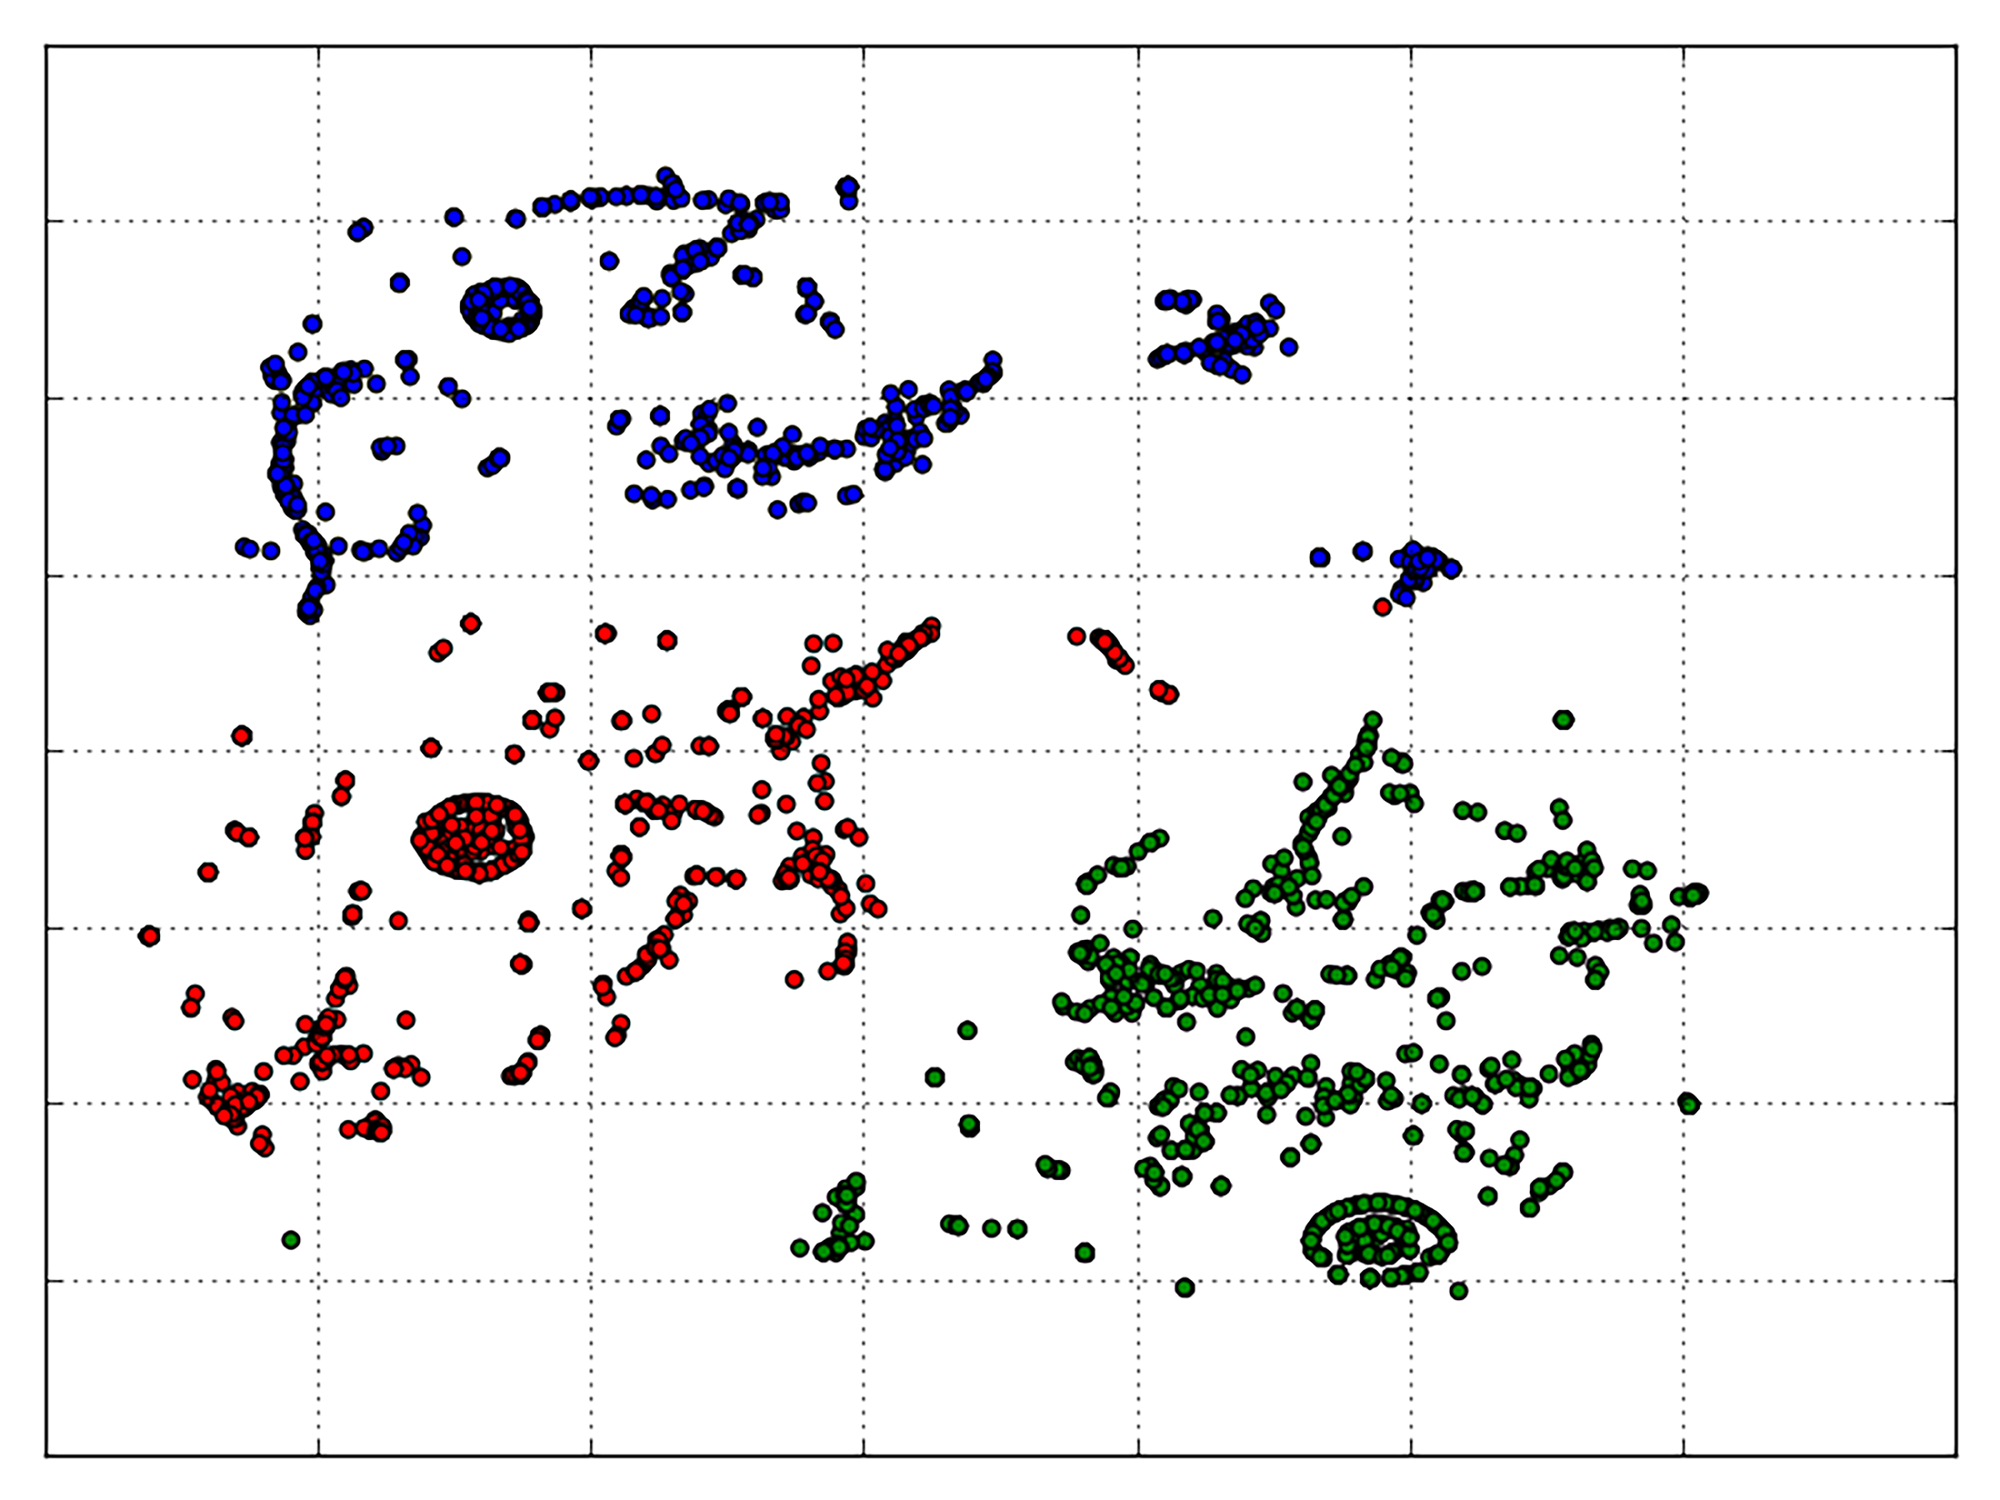
\includegraphics[width=.8\textwidth]{fig/results/context_exact.png}
    \captionsetup{justification=centering}
    \caption{Visualization of context vectors for three different words with different noise seeds using t-SNE}
    \label{fig:context_vector_plot}
\end{figure}

The plot can be seen in Figure \ref{fig:context_vector_plot}, where the three clusters are the words ``PYRAMIDS'' (red), ``MYTHIC'' (blue), and ``SNOWMAN'' (green). We observe that t-SNE places many of the instances of each word in a very focused cluster. However, each word also has instances that are scattered outside their focus areas, indicating a variance in the context vector. We can also see a few examples of extreme outliers for all three words. The low-dimensional visualization indicates that the context vector can retain some of the information in the word itself, despite the applied noise. This is an interesting observation, as it illustrates the robustness of the compression done in the context vector, and how the encoder-decoder can take advantage of this.

\subsection{Decoding}
The decoder and its ability to feed the previous output back as input is one of the corner-stones in the encoder-decoder framework. Allowing the decoder to read the previous output helps the decoder know something about the current state of the ``translation'' process from the vector passed on from the encoder. If the decoder did not feed the output back as input, it would have to rely solely on the hidden states and cell states for the decoding process.

\begin{figure}[ht]
    \centering
    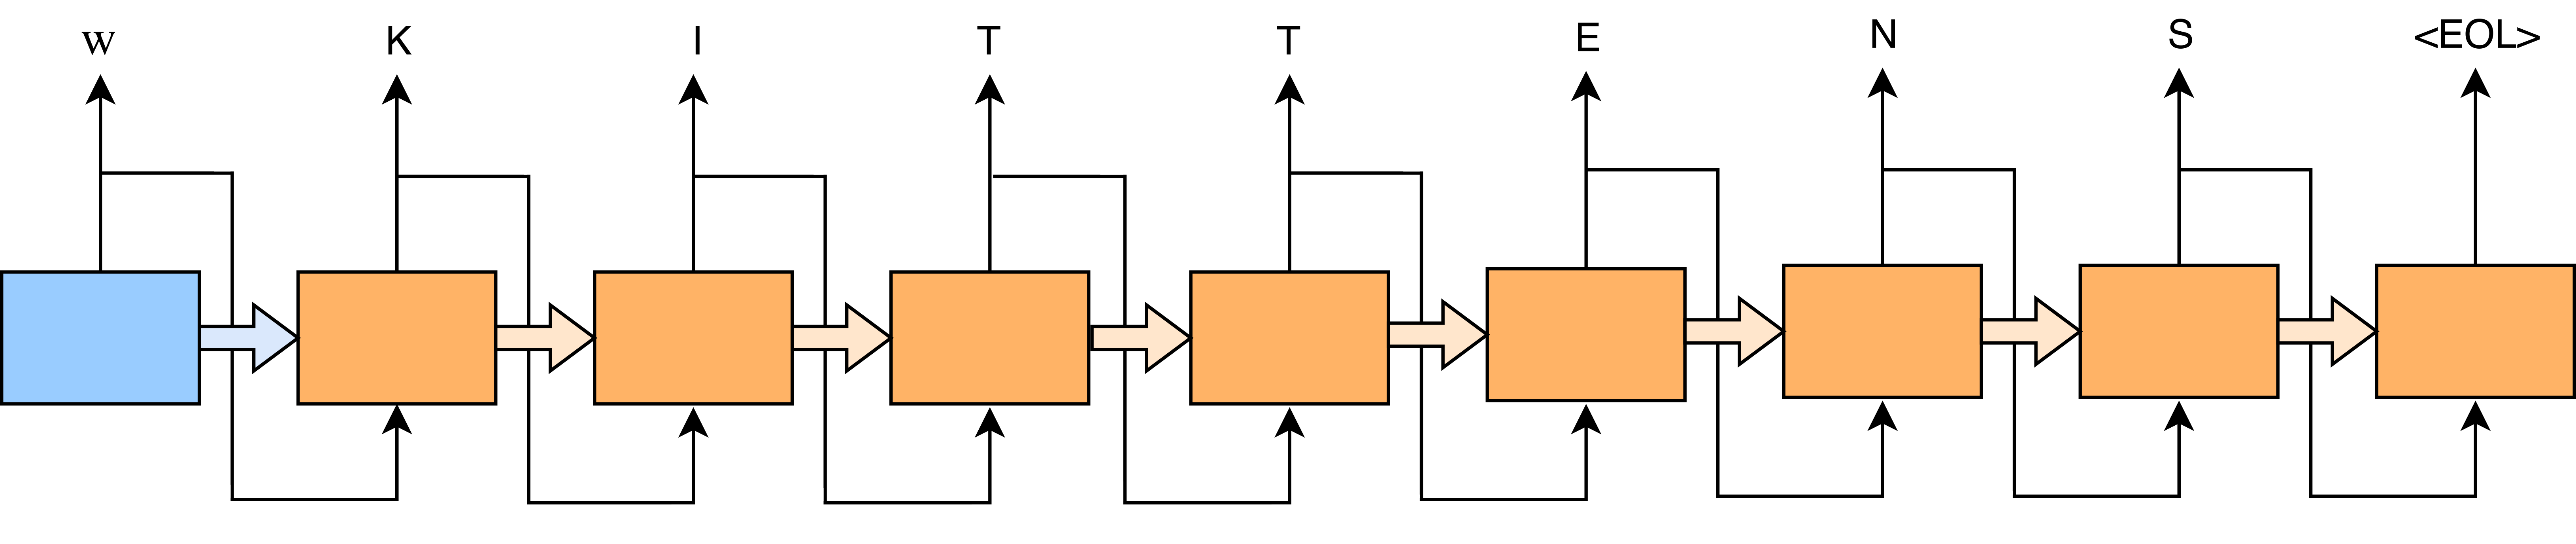
\includegraphics[width=1\textwidth]{fig/results/kittens_correct.png}
    \caption{Decoding the word ``KITTENS''}
    \label{fig:kittens_correct}
\end{figure}

During decoding, the decoder outputs a vector for each timestep, ran through a softmax function. The framework uses {\tt argmax} to find the element in the vector with the highest value, e.i. the predicted value, and feeds this value back to the decoder for the next timestep. We have altered this functionality, and instead of feeding back the predicted value, we send something else back and see how the decoder reacts. Without any modification to the behavior, the model we used is perfectly able to classify each label in the word and produces the correct output ``KITTENS,'' as illustrated in Figure \ref{fig:kittens_correct}. 

\begin{figure}[ht]
    \centering
    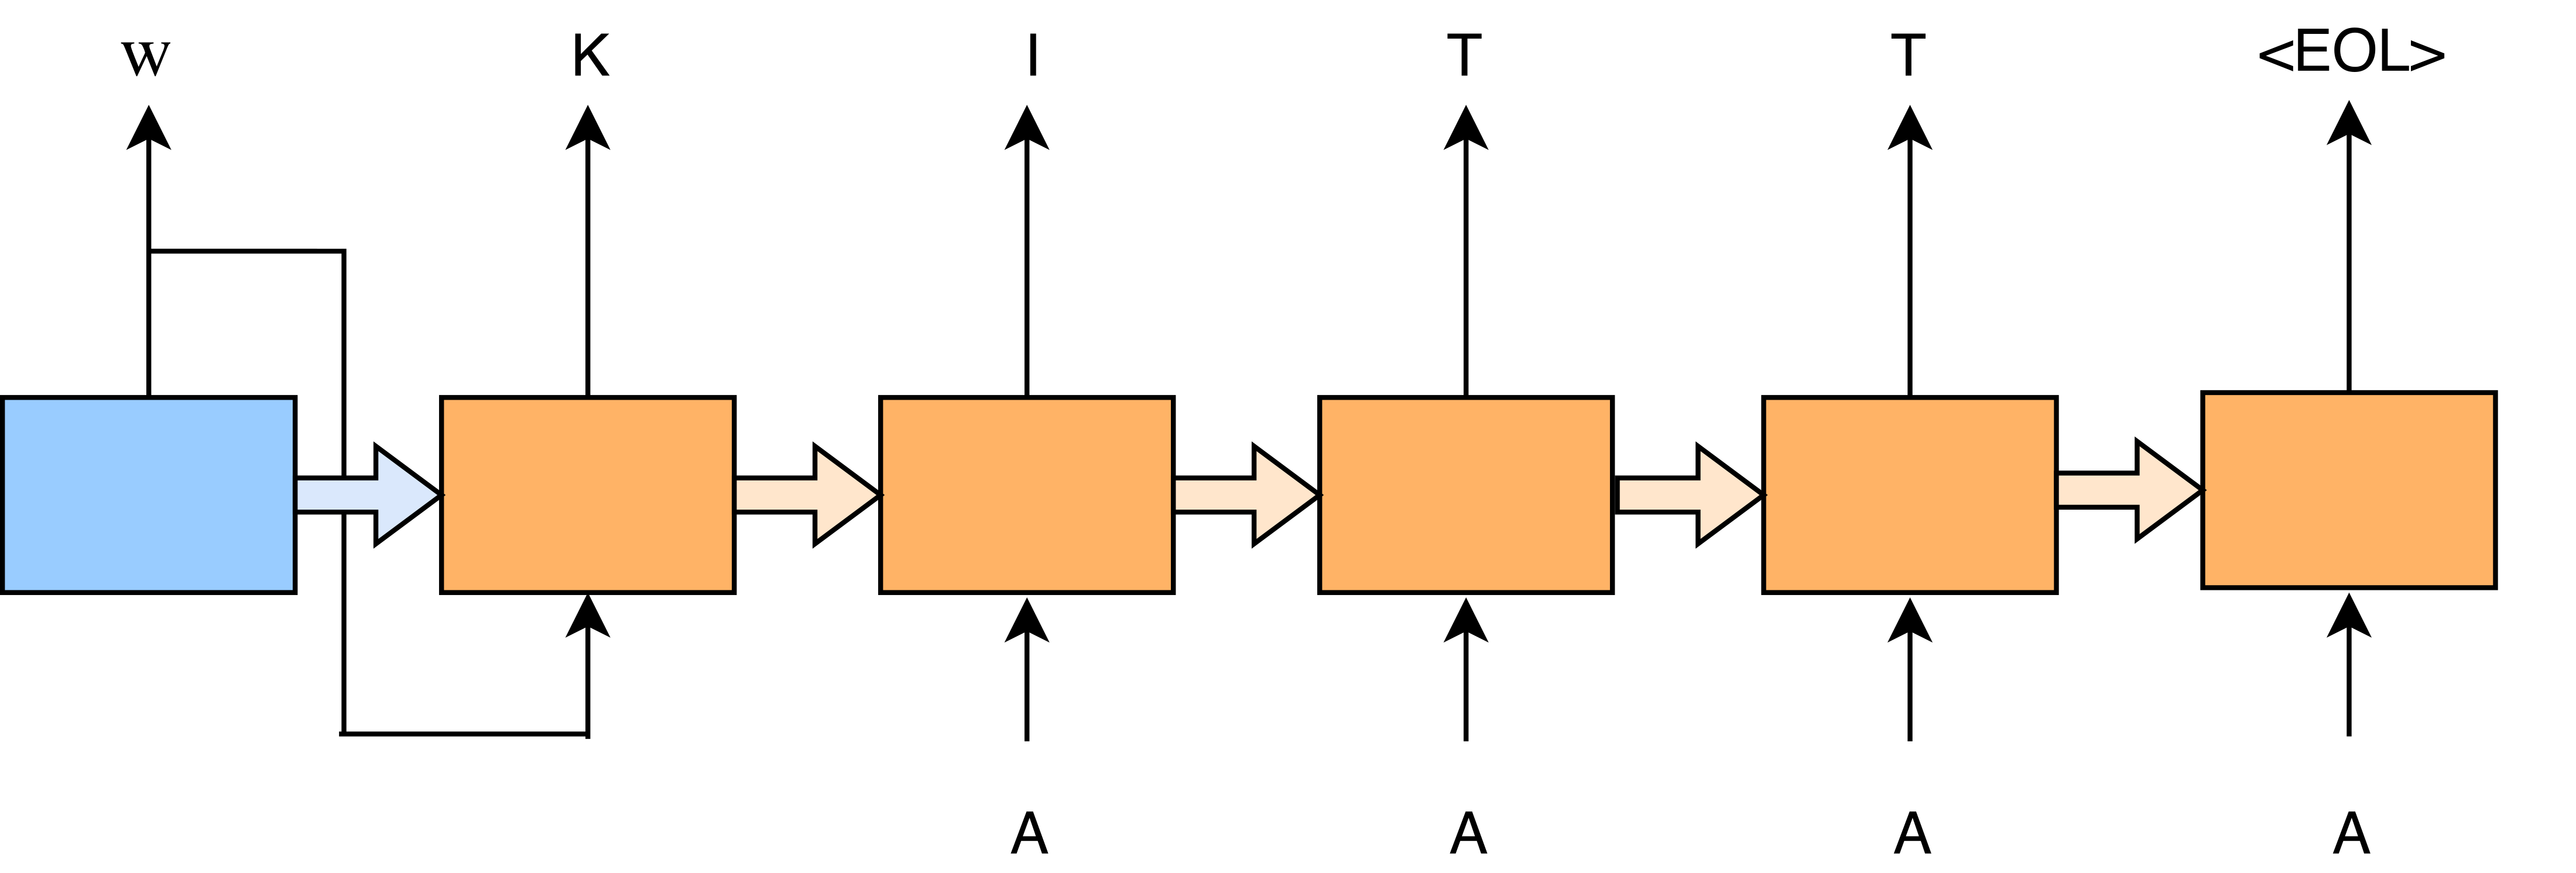
\includegraphics[width=1\textwidth]{fig/results/kittens_wrong.png}
    \caption{Decoding the word ``KITTENS'' by feeding back wrong label}
    \label{fig:kittens_wrong}
\end{figure}

If we instead change the logic to use the {\tt argmin} function, which returns the element we predicted the ``least,'' the word becomes ``KIIIEES.'' Similarly, if we only feed back the first label, which in this case would be the letter A, the word becomes ``KITTT,'' as illustrated in Figure \ref{fig:kittens_wrong}. Note that the first letter in the word is predicted based on the context vector from the encoder, so it is likely this is correct. Except for the first letter, we see some of the other letters in the word have changed. However, despite our trickery, the decoder is still able to predict labels that are actually in the word, indicating the some of the ``knowledge'' in the decoding process is also stored and shared within the recurrent unit. We also observe that the output is not that far off, with both the misled decoders outputting the second letter correctly. Lastly, if we only ``fool'' the decoder for the first and second letter, telling it we outputted an A, the decoder was able to predict every letter correctly, outputting ``KITTENS.'' The correct prediction also indicates that the knowledge in the cell states may correctly override the fed back input, instead of creating a ``domino'' effect as we expected, where the output would progressively get more and more incorrect.

The size of the context vector correlates to the size of the RNN cell, as the context vector is the RNN cell's last hidden state. In the experiments above, the RNN cells had a size of 128. We changed this size to see if this affected the results when we tricked the decoder. The decoder was fed the letter A as the first and second label, similarly to the experiment already carried out, in which the RNN cell with a depth of 128 was able to classify every label correctly. With an RNN cell size of 64, the decoder was still able to classify correctly. However, with a size of 32, the decoder started to misclassify after the first label.

These observations indicate that the encoded context vector contains partial knowledge about which labels to output, especially the first labels. As the decoding progresses, the decoder seems to shift its attention more towards the previous output and relies less on the information from the context vector. Our experiments also indicates that the size of the context vector correlates to how long the decoder can rely on the information in it.

\subsection{Use of Attention}
The experiments carried out in this thesis have shown that both the models based on the encoder-decoder framework were powerful, but the model that utilized the attention mechanism was significantly better. Figure \ref{fig:attention_heatmap} shows the attention heatmap, in other words, the areas in which the attention mechanism focused while classifying each label. In this example, the model correctly classifies the word ``IMAGINED.'' The signature configurations for this experiment was reused from Table \ref{table:signature_sequence_example}.

\begin{figure}[ht]
    \centering
    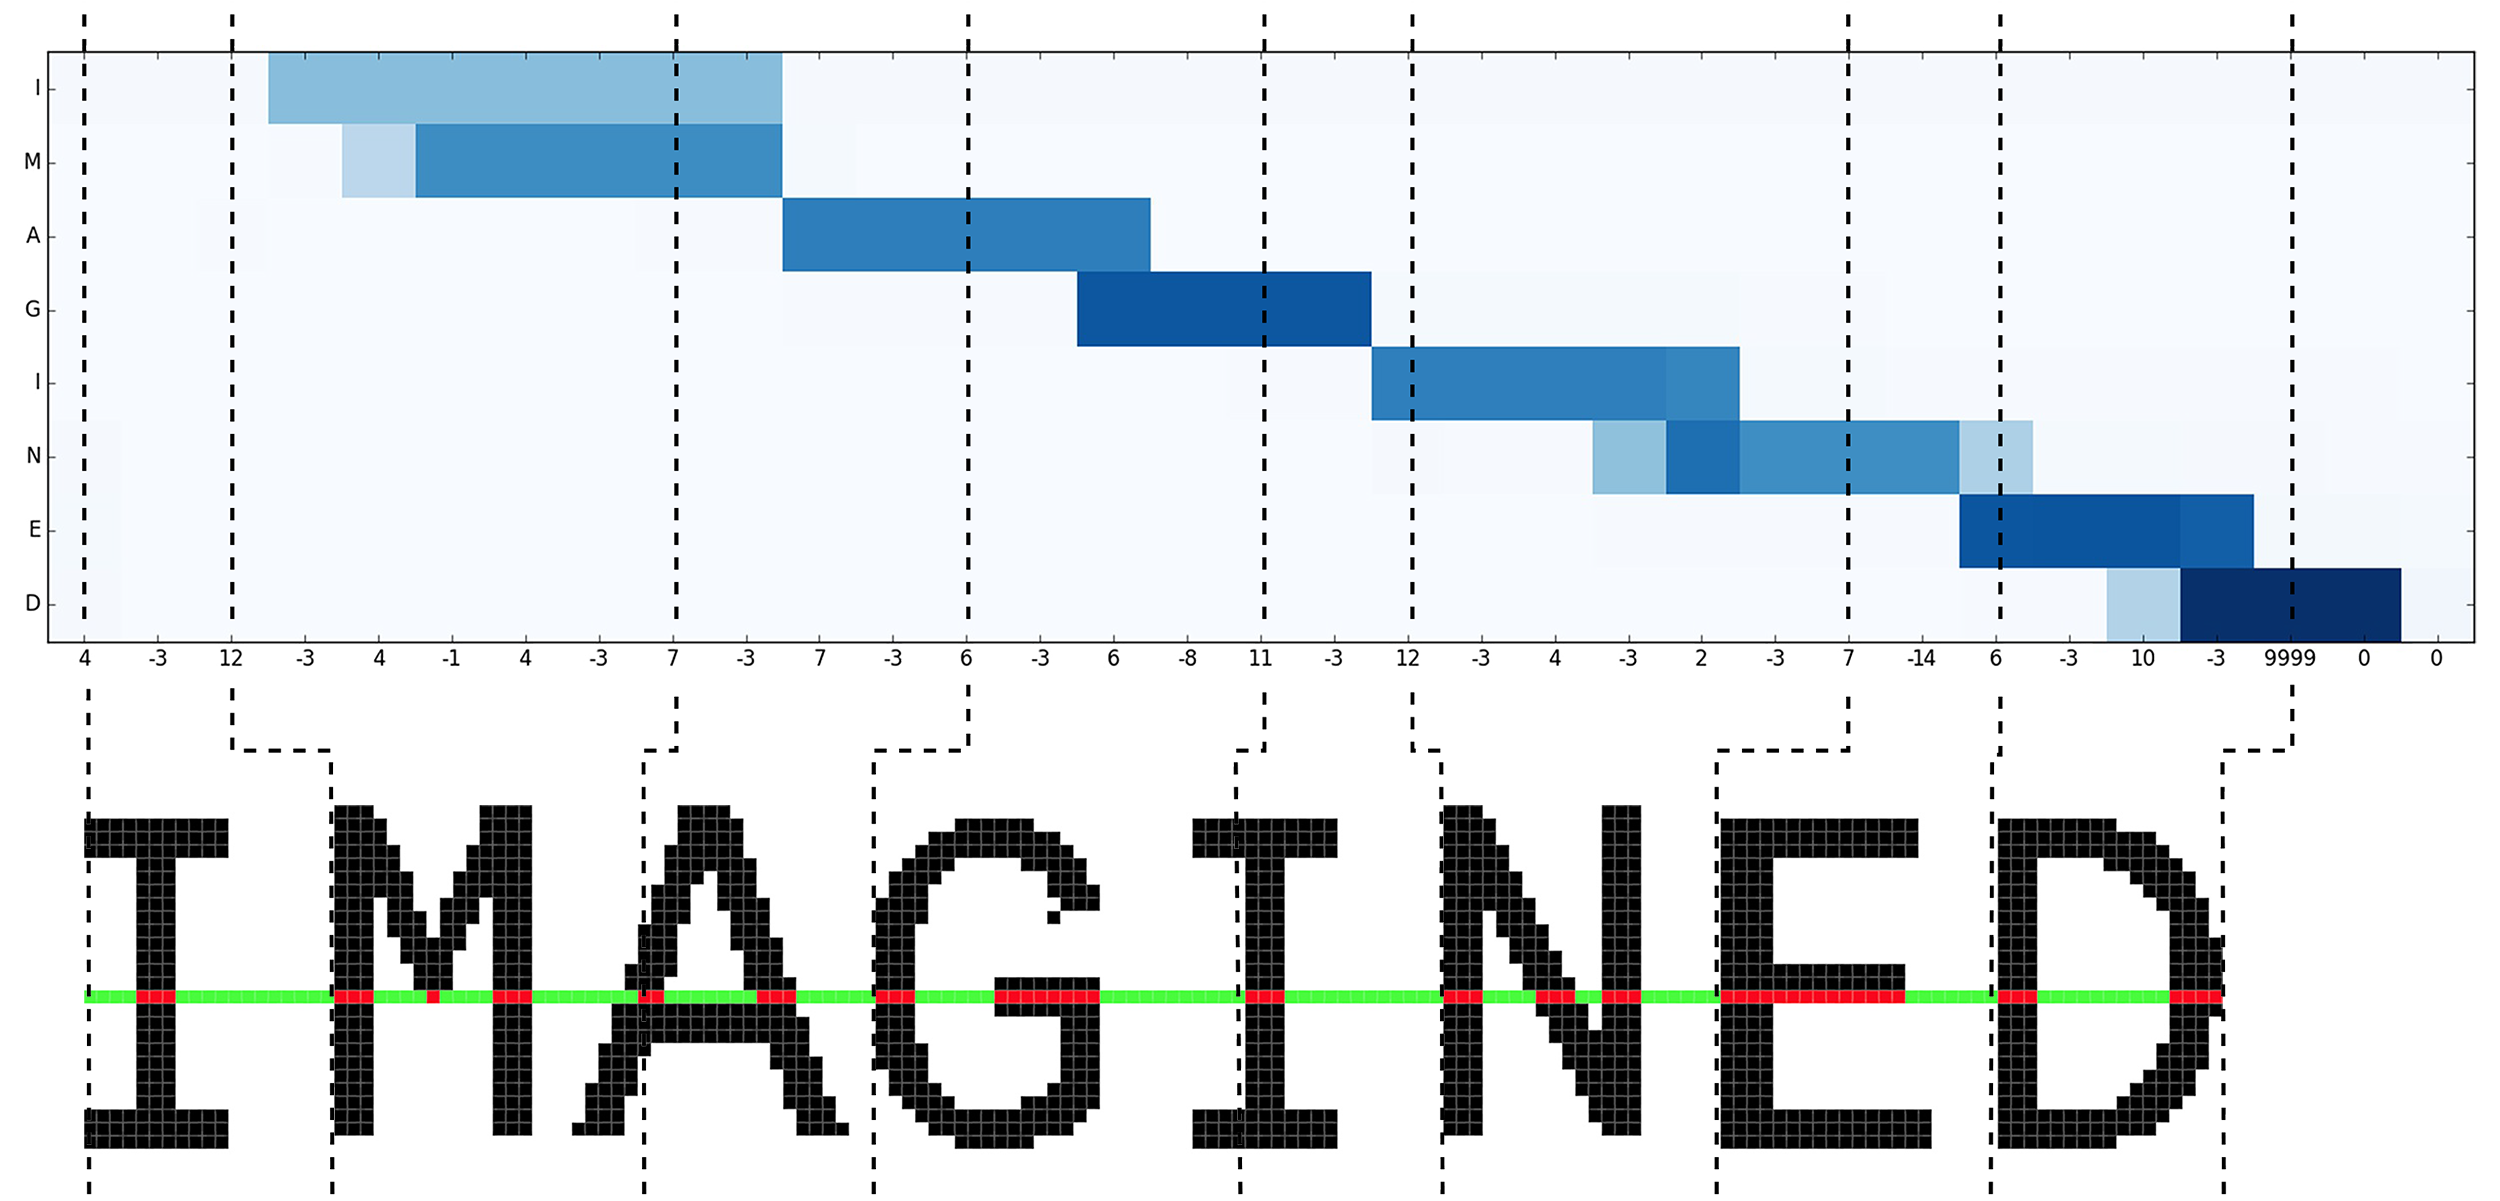
\includegraphics[width=1\textwidth]{fig/conclusion/attention_illustrated.png}
    \caption{Attention heatmap}
    \label{fig:attention_heatmap}
\end{figure}

Some interesting observations can be done with the information from the heatmap and the aligned input text. One interesting observation is that while classifying the very first label, the attention mechanism pays no interest in the values for that label, and only focuses on later values. Table \ref{table:signature_sequence_example} indicates that the signature for the letter I is shared among five other letters, and it may seem like the attention mechanism is smart enough to consider later input to classify the label correctly. We can observe the same behavior when the second I is classified. The signature for the letter E is shared with the letter F, and we observe that the attention mechanism focuses on information beyond its own signature. The attention mechanism most likely does this because the only way to differentiate between and an F and an E is with the sequences after its own signature. The signatures for the letter M and N both begin with the same subsequence \([-3, 4]\). This is reflected in the attention heatmap where we observe that the mechanism pay extensive attention to values after this subsequence while classifying both these letters.

The additional information provided by the attention mechanism gives the {\tt EncDecAtt} model a significant advantage over the {\tt EncDecReg} model, which can only rely on the information in the context vector. We see that this benefit pays off in the consistently better results the {\tt EncDegAtt} model has compared to the {\tt EncDecReg} model. The heatmap also shows how the attention mechanism was able to keep attention fixed on longer subsequences, accounting for the different width ratio between input and output.